% Propuesta técnica · Los Gantt-sters · DGP 2026-2027
% Compila con pdfLaTeX, XeLaTeX o LuaLaTeX (en Overleaf vale el compilador por defecto).
\documentclass[11pt,a4paper]{article}

\usepackage{iftex}
\ifPDFTeX
  \usepackage[T1]{fontenc}
  \usepackage[utf8]{inputenc}
  \usepackage{tgheros}
  \renewcommand{\familydefault}{\sfdefault}
\else
  \usepackage{fontspec}
  \setmainfont{TeX Gyre Heros}
\fi
\usepackage[spanish,es-noshorthands,es-tabla]{babel}
\usepackage[a4paper,top=2.9cm,bottom=2.4cm,left=2.5cm,right=2.5cm,headheight=20pt,headsep=0.8cm]{geometry}
\usepackage[table]{xcolor}
\usepackage{needspace,graphicx,longtable,array,enumitem,titlesec,fancyhdr,caption}
\usepackage{etoolbox,float}
\usepackage[hidelinks]{hyperref}

% ---------- Identidad visual común ----------
\definecolor{gblue}{HTML}{1F4FB4}
\definecolor{gnavy}{HTML}{1B2236}
\definecolor{ggreen}{HTML}{2E9E5B}
\definecolor{ggray}{HTML}{5F6B7A}
\definecolor{gpale}{HTML}{8D919B}
\definecolor{glight}{HTML}{E9EFFB}
\definecolor{gline}{HTML}{B1C1E5}

\newcommand{\proyecto}{Propuesta técnica}
\newcommand{\hl}[1]{\textcolor{gblue}{\textbf{#1}}}
\newcommand{\bloque}[1]{\par\medskip\noindent{\bfseries\color{gnavy}#1}\par\nopagebreak\smallskip}

\color{gnavy}
\setlength{\parindent}{0pt}
\setlength{\parskip}{6pt}
\renewcommand{\baselinestretch}{1.1}
\hypersetup{pdftitle={Propuesta técnica – Los Gantt-sters},pdfauthor={Los Gantt-sters},pdfsubject={Propuesta técnica DGP}}

% Títulos de sección: número en recuadro azul, texto azul y filete verde
\titleformat{\section}{\Large\bfseries\color{gblue}}
  {\colorbox{gblue}{\textcolor{white}{\thesection}}}{0.6em}{}[\vspace{-4pt}{\color{ggreen}\titlerule[0.8pt]}]
\titlespacing*{\section}{0pt}{18pt}{10pt}
\titleformat{\subsection}{\large\bfseries\color{ggreen}}{\thesubsection}{0.6em}{}
\titlespacing*{\subsection}{0pt}{10pt}{4pt}

\setlist[itemize]{label={\color{gblue}\textbullet},leftmargin=1.4em,itemsep=1pt,parsep=0pt,topsep=2pt}
\captionsetup{font={small,it},labelfont={small,it},textfont={color=ggray},labelsep=period}
\setlength{\LTpre}{6pt}\setlength{\LTpost}{8pt}
\renewcommand{\arraystretch}{1.35}
\arrayrulecolor{gline}

% ---------- Objetivos específicos y requisitos ----------
% \objetivo{identificador}{título}{descripción}{historias del Product Backlog}
\newcommand{\objetivo}[4]{%
  \needspace{11\baselineskip}\par\medskip
  \noindent\colorbox{glight}{\parbox{\dimexpr\linewidth-2\fboxsep\relax}{\raggedright\hl{#1. #2}}}\par\nopagebreak
  #3\par\nopagebreak
  {\small\color{ggray}\textit{Historias del Product Backlog relacionadas: #4.}}\par\nopagebreak}
% \grupo{título del grupo de requisitos}
\newcommand{\grupo}[1]{\needspace{3\baselineskip}\par\smallskip\noindent{\small\bfseries\color{ggreen}#1}\par\nopagebreak}
% Lista de requisitos: identificador en azul a la izquierda y texto a la derecha
\newlist{reqs}{description}{1}
\setlist[reqs]{style=multiline,leftmargin=1.85cm,font=\normalfont\small\bfseries\color{gblue},itemsep=1.5pt,parsep=0pt,topsep=1pt,partopsep=0pt,before=\small}

% Cabecera y pie
\pagestyle{fancy}\fancyhf{}
\renewcommand{\headrulewidth}{0pt}
\fancyhead[L]{\raisebox{-0.25\height}{
\includegraphics[height=0.55cm]{logo.png}}\hspace{0.5em}{\small\bfseries\color{gblue}LOS GANTT-STERS}}
\fancyhead[R]{\small\color{ggray}\proyecto\ ·\ Curso 2026-2027}
\fancyfoot[C]{{\color{gpale}\rule{2.5cm}{0.4pt}}\\[2pt]\small\color{ggray}\thepage}

\begin{document}

% ---------- Portada ----------
\begin{titlepage}
\centering
\vspace*{0.2cm}
{\fontsize{30}{34}\selectfont\bfseries\color{gblue}DGP\par}
\vspace{4pt}
{\small\bfseries\color{ggreen}Dirección y Gestión de Proyectos\par}
\vspace{0.8cm}

\includegraphics[width=4.2cm]{logo.png}\par
\vspace{0.9cm}
{\fontsize{24}{28}\selectfont\bfseries\color{gnavy}LOS GANTT-STERS\par}
\vspace{8pt}
{\color{ggreen}\rule{\linewidth}{1.2pt}\par}
\vspace{0.8cm}
{\fontsize{20}{24}\selectfont\bfseries\color{gblue}PROPUESTA TÉCNICA\par}
\vspace{6pt}
{\bfseries\color{gnavy}TUAGENDITA · AGENDA PERSONALIZADA ACCESIBLE\par}
\vspace{1.1cm}
{\footnotesize\bfseries\color{ggray}Integrantes\par}
\vspace{4pt}
{\color{gblue}\rule{\linewidth}{1.2pt}\par}
\vspace{10pt}
\begin{tabular}{c}
Javier Miñán Molina\\[3pt]
Germán Delgado Fernández\\[3pt]
Ana Meca Cano\\[3pt]
Jaime Montávez Ruiz\\[3pt]
Álvaro Sanabria Díaz\\[3pt]
Juan Luis Jiménez Urbano
\end{tabular}\par
\vspace{14pt}
{\small\color{gpale}Universidad de Granada · Curso 2026-2027\par}
\end{titlepage}

% ---------- Ficha ----------
\noindent\begin{tabular}{@{}>{\bfseries\leavevmode\color{gblue}}p{3.4cm}p{\dimexpr\linewidth-3.4cm-2\tabcolsep\relax}@{}}
Proyecto & TuAgendita: agenda personalizada y accesible para estudiantes con discapacidad intelectual (PTVAL) \\ \hline
Cliente & Colegio de Educación Especial Fundación Purísima Concepción (Granada) \\ \hline
Grupo & Los Gantt-sters \\ \hline
Fecha & 15/10/2026 \\ \hline
\end{tabular}\par

\subsection*{El proyecto de un vistazo}
\rowcolors{1}{glight}{white}
\noindent\begin{tabular}{@{}>{\bfseries\leavevmode\color{gblue}}p{4.8cm}p{\dimexpr\linewidth-4.8cm-2\tabcolsep\relax}@{}}
Duración & 2,5 meses, del 1 de octubre al 16 de diciembre de 2026 \\
Tipo de caso de negocio & Demanda, acompañada de un requisito legal \\
Metodología & Scrum: fase inicial y tres iteraciones (sprints) con incremento funcional \\
Gestión de los sprints & Jira \\
Plataforma & Aplicación web (webapp) que se usa desde el navegador: tablets en formato horizontal, móviles y ordenador \\
Tecnologías & Native para el front-end; hosting en Vercel; backend: Supabase \\
Pictogramas & API pública de ARASAAC \\
Normativa & WCAG 2.1 AA, EN 301 549, RGPD y LOPDGDD \\
Objetivos y requisitos & 17 objetivos específicos, con 152 requisitos funcionales, 55 no funcionales y 44 de información \\
Beneficiarios & Alumnado del PTVAL, tutores, familias y personal del Colegio \\
\end{tabular}\par
\rowcolors{1}{}{}
\clearpage

% ---------- Contenido ----------
\section{Título y resumen}
\subsection*{TuAgendita: agenda personalizada y accesible para estudiantes con discapacidad intelectual del Programa de Transición a la Vida Adulta (PTVAL)}
\hl{TuAgendita} es una aplicación web destinada al Colegio de Educación Especial Fundación Purísima Concepción de Granada, cuyo objetivo es facilitar al alumnado del Programa de Transición a la Vida Adulta (PTVAL) la organización y realización de sus actividades diarias. La aplicación permitirá que cada estudiante consulte sus tareas mediante una interfaz visual y accesible, utilizando recursos como pictogramas de ARASAAC, fotografías, audios y vídeos. Además, las tareas podrán dividirse en diferentes pasos que el estudiante podrá ir completando, incorporando un reloj visual para facilitar la percepción del paso del tiempo cuando así lo requiera su perfil.

La aplicación permitirá gestionar tanto las tareas propias del centro —reprografía, comedor, reparto del menú mensual y guía de visitas— como las tareas personales creadas por tutores, familiares o, cuando sus capacidades lo permitan, por los propios estudiantes. Los tutores y administradores podrán configurar individualmente aspectos de la interfaz, como los colores, el tipo y tamaño de letra, el tamaño de los botones, la vista diaria o semanal, el reloj visual y el método de acceso. También dispondrán de herramientas para consultar el progreso del alumnado.

El proyecto será desarrollado por el equipo \hl{Los Gantt-sters}, formado por seis estudiantes del Grado en Ingeniería Informática de la Universidad de Granada, en el marco de las asignaturas DGP y MDA y del proyecto de innovación docente AUTOVIDA. El desarrollo se organizará mediante la metodología Scrum y los sprints se planificarán y seguirán con la aplicación \hl{Jira}. Todo el proyecto se construirá como una \hl{aplicación web}: el front-end se desarrollará con \hl{Native}, se publicará en Vercel y se apoyará en Supabase como backend. La solución tendrá en cuenta desde su diseño los requisitos de accesibilidad y protección de datos aplicables.

\section{Duración}
El proyecto tendrá una duración de \hl{2,5 meses}: comenzará el \hl{1 de octubre de 2026} y finalizará el \hl{16 de diciembre de 2026}.

La planificación de prácticas de la asignatura sitúa la entrega de la tercera iteración el 21 de diciembre de 2026. El equipo fija el \hl{16 de diciembre} como fecha de cierre para disponer de margen ante imprevistos, de acuerdo con la norma interna de tener el trabajo terminado antes de cada entrega oficial.

\needspace{18\baselineskip}
El trabajo se organiza en una fase inicial y \hl{tres iteraciones}, con las fechas que establece el guion de prácticas:

\par\noindent\begin{tabular}{@{}>{\raggedright\arraybackslash}p{\dimexpr 0.2500\linewidth-2\tabcolsep\relax}>{\raggedright\arraybackslash}p{\dimexpr 0.3438\linewidth-2\tabcolsep\relax}>{\raggedright\arraybackslash}p{\dimexpr 0.4062\linewidth-2\tabcolsep\relax}@{}}
\rowcolor{gblue}\textcolor{white}{\textbf{Etapa}} & \textcolor{white}{\textbf{Inicio}} & \textcolor{white}{\textbf{Entrega}} \\
\hl{Fase inicial} & 1 de octubre de 2026 & 21 de octubre de 2026 \\ \arrayrulecolor{gline}\hline
\rowcolor{glight}
\hl{Iteración 1} & 22-23 de octubre de 2026 & 11-12 de noviembre de 2026 \\ \arrayrulecolor{gline}\hline
\hl{Iteración 2} & 12-13 de noviembre de 2026 & 2-3 de diciembre de 2026 \\ \arrayrulecolor{gline}\hline
\rowcolor{glight}
\hl{Iteración 3} & 3-4 de diciembre de 2026 & 16 de diciembre de 2026 (entrega oficial: 21 de diciembre) \\ \arrayrulecolor{gline}\hline
\end{tabular}\par\medskip
Al finalizar la primera y la segunda iteración se realizará una presentación del trabajo desarrollado. Además, a mitad del proyecto se realizará una presentación al cliente, en la fecha y el lugar que se determinen.

\section{Tipo de caso de negocio}
El proyecto se plantea como un caso de \hl{demanda, acompañado de un requisito legal}.

\subsection*{Demanda}
La necesidad surge de una petición real de la dirección del Colegio de Educación Especial Fundación Purísima Concepción, que requiere una herramienta específica para ayudar al alumnado del PTVAL a organizar su tiempo y realizar sus tareas con una mayor autonomía.

Las soluciones actualmente disponibles no cubren completamente las necesidades del centro, debido principalmente a sus limitaciones de accesibilidad para personas con discapacidad cognitiva y a las dificultades o costes asociados a su personalización por parte de los tutores.

\subsection*{Requisito legal}
La aplicación deberá cumplir la normativa aplicable en materia de \hl{accesibilidad y protección de datos}, prestando especial atención al tratamiento de información perteneciente a menores y personas con discapacidad. En particular, se tendrán en cuenta el \hl{Reglamento General de Protección de Datos (RGPD)} y la \hl{LOPDGDD}.

\section{Objetivos}
\subsection*{4.1. Objetivo general}
Desarrollar y entregar antes del \hl{16 de diciembre de 2026} una agenda digital personalizada y accesible, en forma de aplicación web, que permita al alumnado del PTVAL del Colegio Fundación Purísima Concepción organizar y realizar sus tareas diarias con la mayor autonomía posible, proporcionando a los tutores las herramientas necesarias para configurar la agenda y realizar un seguimiento de su progreso.

\subsection*{4.2. Objetivos específicos}
El objetivo general se concreta en \hl{17 objetivos específicos}. Los objetivos OE1 a OE16 describen el producto y cada uno se desglosa en tres tipos de requisitos:

\begin{itemize}
\item \hl{Requisitos funcionales (RF):} todo lo que hace el sistema.
\item \hl{Requisitos no funcionales (RNF):} las condiciones que debe cumplir al hacerlo: accesibilidad, usabilidad, seguridad, compatibilidad y calidad.
\item \hl{Requisitos de información (RI):} los datos que el sistema guarda y gestiona.
\end{itemize}
Cada requisito se identifica con el número de su objetivo: RF3.2 es el segundo requisito funcional del OE3. El objetivo OE17 es de gestión del proyecto y no genera requisitos del sistema.

La tabla resume los objetivos, las historias de usuario del Product Backlog con las que se corresponde cada uno y el número de requisitos de cada tipo.

{\small\par\noindent\begin{tabular}{@{}>{\raggedright\arraybackslash}p{\dimexpr 0.0900\linewidth-2\tabcolsep\relax}>{\raggedright\arraybackslash}p{\dimexpr 0.4300\linewidth-2\tabcolsep\relax}>{\raggedright\arraybackslash}p{\dimexpr 0.2700\linewidth-2\tabcolsep\relax}>{\centering\arraybackslash}p{\dimexpr 0.0700\linewidth-2\tabcolsep\relax}>{\centering\arraybackslash}p{\dimexpr 0.0700\linewidth-2\tabcolsep\relax}>{\centering\arraybackslash}p{\dimexpr 0.0700\linewidth-2\tabcolsep\relax}@{}}
\rowcolor{gblue}\textcolor{white}{\textbf{N.º}} & \textcolor{white}{\textbf{Objetivo específico}} & \textcolor{white}{\textbf{Historias (Práctica 2)}} & \textcolor{white}{\textbf{RF}} & \textcolor{white}{\textbf{RNF}} & \textcolor{white}{\textbf{RI}} \\
\hl{OE1} & Acceso y autenticación adaptada & HU-01, HU-02 & 9 & 4 & 3 \\ \arrayrulecolor{gline}\hline
\rowcolor{glight}
\hl{OE2} & Gestión de usuarios, roles y vínculos & HU-03 & 13 & 3 & 5 \\ \arrayrulecolor{gline}\hline
\hl{OE3} & Personalización del perfil y de la interfaz & HU-04, HU-05, HU-17 & 17 & 4 & 2 \\ \arrayrulecolor{gline}\hline
\rowcolor{glight}
\hl{OE4} & Agenda y estructuración temporal & HU-06, HU-16, HU-17 & 9 & 4 & 2 \\ \arrayrulecolor{gline}\hline
\hl{OE5} & Tareas personales y tareas por pasos & HU-07, HU-10 & 15 & 3 & 4 \\ \arrayrulecolor{gline}\hline
\rowcolor{glight}
\hl{OE6} & Ejecución guiada de tareas y reloj visual & HU-08, HU-09 & 10 & 4 & 3 \\ \arrayrulecolor{gline}\hline
\hl{OE7} & Tarea del centro: reprografía & HU-14 & 8 & 2 & 2 \\ \arrayrulecolor{gline}\hline
\rowcolor{glight}
\hl{OE8} & Tarea del centro: comedor & HU-11, HU-12 & 11 & 2 & 3 \\ \arrayrulecolor{gline}\hline
\hl{OE9} & Tarea del centro: menú mensual & HU-13 & 7 & 2 & 2 \\ \arrayrulecolor{gline}\hline
\rowcolor{glight}
\hl{OE10} & Tarea del centro: guía de visita & HU-15 & 9 & 2 & 3 \\ \arrayrulecolor{gline}\hline
\hl{OE11} & Necesidades, urgencias y comunicación & HU-18, HU-19, HU-21 & 10 & 3 & 4 \\ \arrayrulecolor{gline}\hline
\rowcolor{glight}
\hl{OE12} & Imprevistos: plan B, prioridad y bloqueo & HU-22, HU-23 & 9 & 2 & 3 \\ \arrayrulecolor{gline}\hline
\hl{OE13} & Seguimiento del progreso & HU-25 & 7 & 3 & 2 \\ \arrayrulecolor{gline}\hline
\rowcolor{glight}
\hl{OE14} & Accesibilidad y usabilidad & HUT-03 y transversal & 7 & 6 & 2 \\ \arrayrulecolor{gline}\hline
\hl{OE15} & Protección de datos y seguridad & HU-03 y transversal & 6 & 5 & 2 \\ \arrayrulecolor{gline}\hline
\rowcolor{glight}
\hl{OE16} & Plataforma web y despliegue & HUT-01, HUT-02, HUT-03 & 5 & 6 & 2 \\ \arrayrulecolor{gline}\hline
\hl{OE17} & Gestión del proyecto & No aplica & -- & -- & -- \\ \arrayrulecolor{gline}\hline
\hl{Total} & & & \textbf{152} & \textbf{55} & \textbf{44} \\ \arrayrulecolor{gline}\hline
\end{tabular}\par}\medskip

Los requisitos proceden del pliego, de la entrevista con el profesorado en su papel de cliente, de los personajes y escenarios de la Práctica 1 y del Product Backlog de la Práctica 2. Las medidas concretas que aparecen en los requisitos no funcionales (tamaños mínimos, tiempos de pulsación y de aviso) son las de los criterios de aceptación de la Práctica 2.

\needspace{16\baselineskip}
\subsection*{4.3. Requisitos de cada objetivo específico}
\objetivo{OE1}{Acceso y autenticación adaptada}{Permitir que cada usuario entre en la aplicación web con un método de acceso adecuado a sus capacidades: el alumnado, sin necesidad de leer ni escribir; el personal supervisor, con credenciales.}{HU-01, HU-02}
\grupo{Requisitos funcionales (RF)}
\begin{reqs}
\item[RF1.1] El sistema mostrará al estudiante una pantalla de bienvenida con las fotografías o pictogramas de los estudiantes de su aula, para que inicie sesión tocando la suya sin escribir ninguna contraseña.
\item[RF1.2] El sistema permitirá el acceso con usuario y contraseña como método alternativo para los estudiantes cuyo perfil lo tenga configurado.
\item[RF1.3] El sistema permitirá a administradores, tutores, familias y especialistas iniciar sesión con correo electrónico y contraseña.
\item[RF1.4] Tras la autenticación, el sistema llevará a cada usuario a la interfaz que corresponde a su rol: la agenda, en el caso del estudiante, o el panel de gestión, en el caso de los supervisores.
\item[RF1.5] El tutor o el administrador podrá elegir, para cada estudiante, el método de acceso que utilizará.
\item[RF1.6] Cuando un dispositivo esté asignado a un único estudiante, el sistema abrirá directamente su sesión personal.
\item[RF1.7] Al tocar su fotografía, el estudiante recibirá una confirmación visual y, si su perfil lo permite, sonora antes de entrar en su agenda.
\item[RF1.8] El sistema permitirá cerrar la sesión.
\item[RF1.9] Si los datos de acceso son incorrectos, el sistema mostrará un mensaje que indique qué dato ha fallado: el correo electrónico o la contraseña.
\end{reqs}
\grupo{Requisitos no funcionales (RNF)}
\begin{reqs}
\item[RNF1.1] Las tarjetas de acceso del estudiante medirán al menos 120~$\times$~120~px e incluirán su nombre en Lectura Fácil.
\item[RNF1.2] El acceso por fotografía o pictograma se completará sin teclado.
\item[RNF1.3] Las contraseñas no se guardarán en claro y las sesiones se gestionarán con los tokens seguros del servicio de autenticación del backend.
\item[RNF1.4] Toda la comunicación entre el navegador y el backend se cifrará mediante HTTPS.
\end{reqs}
\grupo{Requisitos de información (RI)}
\begin{reqs}
\item[RI1.1] Credenciales de acceso: identificador de usuario, correo electrónico (supervisores), contraseña cifrada y método de acceso configurado.
\item[RI1.2] Imagen de acceso del estudiante: fotografía o pictograma y nombre visible.
\item[RI1.3] Sesión: usuario, rol, dispositivo asignado (si procede) y fecha y hora de inicio.
\end{reqs}

\objetivo{OE2}{Gestión de usuarios, roles y vínculos}{Disponer de una gestión centralizada de las personas que usan la aplicación, de sus roles y de la relación entre cada estudiante y quienes lo tutorizan en el centro y en casa.}{HU-03}
\grupo{Requisitos funcionales (RF)}
\begin{reqs}
\item[RF2.1] El administrador podrá dar de alta usuarios con los roles de administrador, tutor, familia, especialista y estudiante.
\item[RF2.2] El administrador podrá consultar los datos de cualquier usuario.
\item[RF2.3] El administrador podrá modificar los datos de cualquier usuario.
\item[RF2.4] El administrador podrá dar de baja a cualquier usuario.
\item[RF2.5] Al registrar un tutor, el sistema guardará quién ejerce esa función: docente del aula, familiar o terapeuta.
\item[RF2.6] Cualquier perfil supervisor podrá dar de alta estudiantes indicando su nombre, su aula y su fotografía.
\item[RF2.7] Solo el administrador y los perfiles de tutor o familia podrán dar de alta tutores.
\item[RF2.8] El sistema permitirá vincular a cada estudiante con su tutor de aula.
\item[RF2.9] El sistema permitirá vincular a cada estudiante con un único tutor familiar.
\item[RF2.10] El sistema organizará a los estudiantes por aulas.
\item[RF2.11] El sistema permitirá consultar la lista de estudiantes de cada aula.
\item[RF2.12] El tutor familiar solo podrá gestionar las tareas del hogar de los estudiantes vinculados con él.
\item[RF2.13] El tutor escolar solo podrá gestionar las tareas del centro de los estudiantes vinculados con él.
\end{reqs}
\grupo{Requisitos no funcionales (RNF)}
\begin{reqs}
\item[RNF2.1] Los permisos por rol se aplicarán también en el backend, con reglas de acceso a los datos, y no solo en la interfaz.
\item[RNF2.2] El panel de gestión podrá utilizarse sin conocimientos técnicos avanzados: formularios guiados, validación de los datos y mensajes de error claros.
\item[RNF2.3] El panel estará optimizado para el navegador del ordenador del aula y será utilizable también en tableta.
\end{reqs}
\grupo{Requisitos de información (RI)}
\begin{reqs}
\item[RI2.1] Usuario: identificador, nombre, rol, estado (activo o inactivo) y fecha de alta.
\item[RI2.2] Estudiante: identificador, nombre, fotografía, aula y código de expediente seudonimizado.
\item[RI2.3] Tutor: identificador, nombre, tipo (docente, familiar o terapeuta) y ámbito de sus permisos (centro u hogar).
\item[RI2.4] Vínculo entre tutor y estudiante: tutor, estudiante, tipo de vínculo (de aula o familiar; como máximo un tutor familiar por estudiante) y fecha.
\item[RI2.5] Aula: identificador, nombre, tutor responsable y estudiantes que la forman.
\end{reqs}

\objetivo{OE3}{Personalización del perfil y de la interfaz}{Adaptar la interfaz a cada estudiante para que el tutor pueda ajustarla a sus necesidades sensoriales, cognitivas y motoras.}{HU-04, HU-05, HU-17}
\grupo{Requisitos funcionales (RF)}
\begin{reqs}
\item[RF3.1] El tutor podrá elegir para cada estudiante la paleta de colores de la interfaz entre al menos tres opciones (clara, oscura y pastel), con una variante de alto contraste.
\item[RF3.2] El tutor podrá elegir el tipo de letra.
\item[RF3.3] El tutor podrá elegir el tamaño de la letra.
\item[RF3.4] El tutor podrá elegir el tamaño de los botones entre al menos tres opciones.
\item[RF3.5] El tutor podrá elegir la forma de los botones.
\item[RF3.6] El tutor podrá elegir la vista de la agenda de cada estudiante: diaria o semanal.
\item[RF3.7] El tutor podrá elegir si el reloj visual se muestra o se oculta.
\item[RF3.8] El tutor podrá dejar el reloj visual fijo en pantalla.
\item[RF3.9] El tutor podrá activar el reloj visual con sonido o sin sonido.
\item[RF3.10] El tutor podrá activar o desactivar los sonidos de la aplicación.
\item[RF3.11] El tutor podrá configurar los avisos para que sean solo visuales.
\item[RF3.12] El tutor podrá habilitar o deshabilitar que el estudiante cree tareas personales.
\item[RF3.13] El tutor podrá habilitar o deshabilitar que el estudiante modifique sus propias preferencias.
\item[RF3.14] El estudiante con permiso podrá elegir, entre las opciones que su tutor deje disponibles, la que prefiera.
\item[RF3.15] Los cambios que guarde el tutor se aplicarán en la sesión abierta del estudiante sin que tenga que volver a entrar.
\item[RF3.16] El sistema ofrecerá un modo de barrido que resalta los elementos de la pantalla uno a uno y permite seleccionarlos con un pulsador externo.
\item[RF3.17] El tutor podrá configurar la velocidad del modo de barrido.
\end{reqs}
\grupo{Requisitos no funcionales (RNF)}
\begin{reqs}
\item[RNF3.1] Los pictogramas y las fotografías serán los mismos para todos los usuarios, para mantener la consistencia visual.
\item[RNF3.2] Todas las paletas ofrecidas cumplirán el contraste mínimo del nivel AA de las WCAG 2.1.
\item[RNF3.3] La configuración de un perfil se completará desde una única pantalla del panel, sin pasos técnicos.
\item[RNF3.4] El modo de barrido permitirá completar cualquier tarea con un único pulsador y sin gestos táctiles.
\end{reqs}
\grupo{Requisitos de información (RI)}
\begin{reqs}
\item[RI3.1] Preferencias de visualización del estudiante: paleta, tipo y tamaño de letra, tamaño y forma de los botones, vista de la agenda, configuración del reloj visual, tipo de avisos y visibilidad del indicador de foco.
\item[RI3.2] Permisos del perfil: si puede crear tareas, si puede modificar sus preferencias, y si usa el modo de barrido y a qué velocidad.
\end{reqs}

\objetivo{OE4}{Agenda del estudiante y estructuración temporal}{Mostrar a cada estudiante qué tiene que hacer ahora y qué viene después, para que pueda anticipar su jornada y reducir la ansiedad ante los cambios de actividad.}{HU-06, HU-16, HU-17}
\grupo{Requisitos funcionales (RF)}
\begin{reqs}
\item[RF4.1] El sistema mostrará al estudiante sus tareas del día en orden cronológico, en tarjetas con pictograma o fotografía, título y hora.
\item[RF4.2] La vista diaria se organizará en tres bloques: «Hecho» (la última tarea completada), «Ahora» (la tarea actual) y «Después» (la siguiente tarea).
\item[RF4.3] Cuando el estudiante confirme el fin de la tarea actual, el sistema la pasará a «Hecho» y moverá la siguiente a «Ahora».
\item[RF4.4] Al pulsar una tarjeta, el sistema abrirá el detalle de la tarea con su descripción accesible: texto, audio, vídeo o secuencia de pasos.
\item[RF4.5] El sistema ofrecerá una vista semanal a los estudiantes que la tengan habilitada.
\item[RF4.6] El sistema permitirá alternar entre la vista diaria y la semanal.
\item[RF4.7] Cinco minutos antes de la siguiente tarea, el sistema mostrará un aviso con su pictograma, sin interrumpir la actividad en curso.
\item[RF4.8] El aviso anticipatorio se cerrará al tocarlo o pasados 15 segundos.
\item[RF4.9] La agenda se actualizará sin recargar la página cuando un tutor cree, modifique, bloquee o cancele una tarea.
\end{reqs}
\grupo{Requisitos no funcionales (RNF)}
\begin{reqs}
\item[RNF4.1] La vista diaria no tendrá barras de desplazamiento ni elementos accesorios, y el bloque «Ahora» ocupará la zona central y más grande de la pantalla.
\item[RNF4.2] El diseño dará prioridad a la tableta en posición horizontal y será funcional también en vertical y en móvil.
\item[RNF4.3] Los avisos podrán configurarse como solo visuales y ninguno usará sonidos estridentes.
\item[RNF4.4] Los textos de la agenda estarán en Lectura Fácil y cada tarea se mostrará siempre con un pictograma o una fotografía.
\end{reqs}
\grupo{Requisitos de información (RI)}
\begin{reqs}
\item[RI4.1] Entrada de la agenda: estudiante, tarea, fecha, hora de inicio, duración prevista, orden y estado (pendiente, en curso, hecha, cancelada o bloqueada).
\item[RI4.2] Aviso anticipatorio: estudiante, tarea, antelación, tipo (visual o sonoro) y hora de emisión.
\end{reqs}

\objetivo{OE5}{Tareas personales y tareas por pasos}{Permitir que tutores, familias y, cuando su perfil lo permita, los propios estudiantes creen tareas personales del centro o del hogar con una descripción accesible.}{HU-07, HU-10}
\grupo{Requisitos funcionales (RF)}
\begin{reqs}
\item[RF5.1] Los tutores y las familias podrán crear tareas personales indicando el nombre, la imagen o pictograma, la hora, la duración y los días de la semana en los que se repite.
\item[RF5.2] El sistema permitirá describir cada tarea con texto, audio, vídeo o una secuencia de pasos.
\item[RF5.3] Cada paso de una tarea tendrá una imagen o pictograma, un texto breve y, de forma opcional, un audio o un vídeo.
\item[RF5.4] El sistema permitirá cambiar el orden de los pasos de una tarea.
\item[RF5.5] El formulario de creación incluirá un buscador de pictogramas de ARASAAC.
\item[RF5.6] El sistema permitirá grabar audio con el micrófono del dispositivo desde el propio navegador.
\item[RF5.7] El sistema permitirá grabar vídeo con la cámara del dispositivo desde el propio navegador.
\item[RF5.8] El sistema permitirá hacer fotografías con la cámara del dispositivo desde el propio navegador.
\item[RF5.9] El sistema permitirá subir archivos de imagen, audio y vídeo ya existentes.
\item[RF5.10] El estudiante con el permiso habilitado podrá crear sus propias tareas con un asistente guiado en el que elige un pictograma por categorías, graba un audio o un vídeo y selecciona el día y la hora de forma visual.
\item[RF5.11] El tutor podrá asignar una misma tarea a varios de los estudiantes que tutoriza.
\item[RF5.12] El tutor podrá modificar las tareas que ha creado.
\item[RF5.13] El tutor podrá eliminar las tareas que ha creado.
\item[RF5.14] El estudiante podrá modificar o cancelar una tarea solo si la prioridad de la tarea lo permite (OE12).
\item[RF5.15] Las tareas creadas por el estudiante se mostrarán en modo consulta a su tutor escolar y a su tutor familiar.
\end{reqs}
\grupo{Requisitos no funcionales (RNF)}
\begin{reqs}
\item[RNF5.1] Crear una tarea no exigirá al estudiante escribir texto.
\item[RNF5.2] Los archivos de audio, vídeo e imagen se comprimirán antes de almacenarse.
\item[RNF5.3] Cada recurso multimedia tendrá una descripción textual alternativa.
\end{reqs}
\grupo{Requisitos de información (RI)}
\begin{reqs}
\item[RI5.1] Tarea: identificador, nombre, tipo (personal del centro, del hogar o propia del centro), pictograma o imagen, descripción, creador, prioridad, hora, duración y días de repetición.
\item[RI5.2] Paso: tarea, orden, texto, imagen, audio y vídeo.
\item[RI5.3] Asignación: tarea, estudiante, persona que la asigna y fecha.
\item[RI5.4] Recurso multimedia: tipo, archivo, descripción alternativa, origen (ARASAAC o propio) y autor.
\end{reqs}

\objetivo{OE6}{Ejecución guiada de tareas y reloj visual}{Guiar al estudiante mientras realiza una tarea, registrar su avance y ayudarle a percibir el paso del tiempo sin generarle ansiedad.}{HU-08, HU-09}
\grupo{Requisitos funcionales (RF)}
\begin{reqs}
\item[RF6.1] El sistema mostrará en la tarea actual un botón «Empezar» que la pone en curso, registra la hora de inicio y activa el reloj visual.
\item[RF6.2] En las tareas por pasos, el sistema mostrará un paso cada vez y el estudiante confirmará cada uno; no se podrá avanzar al paso siguiente sin confirmar el anterior.
\item[RF6.3] El estudiante podrá reproducir el audio o el vídeo de cada paso tantas veces como quiera.
\item[RF6.4] El sistema mostrará un botón «Terminar» que registra la hora de fin y marca la tarea como completada.
\item[RF6.5] Al completar una tarea, el sistema mostrará un refuerzo positivo: una animación, un pictograma y, si el perfil lo permite, un sonido.
\item[RF6.6] En las tareas con duración conocida, el sistema mostrará un reloj visual: un disco de color que se reduce de forma proporcional al tiempo que queda.
\item[RF6.7] Si el perfil lo tiene activado, el reloj visual mostrará debajo un rótulo en Lectura Fácil con el tiempo restante (por ejemplo, «Quedan 10 minutos»).
\item[RF6.8] Cuando se agote el tiempo, el sistema lo indicará con un aviso visual suave y, si el perfil lo permite, con un sonido suave.
\item[RF6.9] El tutor podrá marcar una tarea para que sea obligatorio registrar su inicio y su fin.
\item[RF6.10] Desde el detalle de una tarea, el estudiante podrá escanear con la cámara el código QR de apoyo de la sala y el sistema mostrará el contenido de apoyo asociado a esa sala.
\end{reqs}
\grupo{Requisitos no funcionales (RNF)}
\begin{reqs}
\item[RNF6.1] Los botones «Empezar» y «Terminar» exigirán una pulsación mantenida de 1,5 segundos o una confirmación simple, para evitar toques accidentales.
\item[RNF6.2] El reloj visual no emitirá tictac ni pitidos y podrá dejarse fijo en pantalla.
\item[RNF6.3] Todos los controles tendrán un área táctil de al menos 48~$\times$~48~px.
\item[RNF6.4] Durante la ejecución de una tarea no habrá campos de texto libre para el estudiante.
\end{reqs}
\grupo{Requisitos de información (RI)}
\begin{reqs}
\item[RI6.1] Registro de ejecución: estudiante, tarea, fecha, hora de inicio, hora de fin y estado final.
\item[RI6.2] Registro de pasos: ejecución, paso y hora de confirmación.
\item[RI6.3] Código QR de sala: sala, código y contenido de apoyo asociado.
\end{reqs}

\objetivo{OE7}{Tarea del centro: reprografía}{Permitir que un estudiante complete de forma autónoma un encargo de reprografía, desde que recoge el material hasta que lo entrega.}{HU-14}
\grupo{Requisitos funcionales (RF)}
\begin{reqs}
\item[RF7.1] Un docente o el encargado del taller podrá registrar un encargo de reprografía indicando el aula de origen, el trabajo solicitado (fotocopiar, plastificar o encuadernar) y la cantidad.
\item[RF7.2] El encargado del taller o el administrador podrá asignar el encargo a un estudiante.
\item[RF7.3] Al asignar el encargo, el sistema lo añadirá a la agenda del estudiante.
\item[RF7.4] El sistema guiará al estudiante en tres fases: recogida del material en el aula, trabajo en el taller y entrega en el aula; cada fase tendrá su pictograma, su texto y su botón de confirmación.
\item[RF7.5] El sistema no permitirá pasar a la fase siguiente sin confirmar la anterior.
\item[RF7.6] Al confirmar la entrega, el sistema marcará el encargo como completado.
\item[RF7.7] Al completarse el encargo, el sistema lo notificará al docente que lo solicitó.
\item[RF7.8] El docente solicitante y el encargado del taller podrán consultar en qué fase se encuentra cada encargo.
\end{reqs}
\grupo{Requisitos no funcionales (RNF)}
\begin{reqs}
\item[RNF7.1] La navegación será estrictamente lineal y el estudiante no tendrá que escribir texto.
\item[RNF7.2] Cada fase se presentará con un pictograma de ARASAAC y un texto en Lectura Fácil.
\end{reqs}
\grupo{Requisitos de información (RI)}
\begin{reqs}
\item[RI7.1] Encargo de reprografía: solicitante, aula de origen, aula de entrega, tipo de trabajo, número de copias, fecha, estudiante asignado y fase actual.
\item[RI7.2] Registro de fases: encargo, fase y hora de confirmación.
\end{reqs}

\objetivo{OE8}{Tarea del centro: comedor}{Permitir que un estudiante recoja cada día, aula por aula, quién se queda al comedor y con qué dieta, y que el parte llegue a cocina sin errores de transcripción.}{HU-11, HU-12}
\grupo{Requisitos funcionales (RF)}
\begin{reqs}
\item[RF8.1] El tutor establecerá el tipo de dieta de cada estudiante: basal, túrmix, texturizada, cetogénica u otras que defina el centro.
\item[RF8.2] El administrador asignará la tarea diaria de comedor a un estudiante.
\item[RF8.3] El sistema mostrará al estudiante encargado, aula por aula, la lista de estudiantes con su fotografía para que marque quién se queda al comedor y quién está ausente.
\item[RF8.4] Para cada comensal, el sistema aplicará la dieta que ha configurado su tutor y la mostrará con su pictograma para que el encargado la confirme.
\item[RF8.5] El sistema permitirá pasar al siguiente estudiante o cambiar de aula.
\item[RF8.6] El sistema mostrará qué aulas están ya completadas.
\item[RF8.7] Al terminar la última aula, el sistema mostrará un resumen con el número de comensales de cada tipo de dieta.
\item[RF8.8] El estudiante enviará el parte a cocina con una sola pulsación.
\item[RF8.9] El personal de cocina consultará el parte en una vista propia.
\item[RF8.10] El personal de cocina podrá exportar el parte.
\item[RF8.11] El sistema guardará el registro diario de comensales.
\end{reqs}
\grupo{Requisitos no funcionales (RNF)}
\begin{reqs}
\item[RNF8.1] Toda la tarea podrá completarse con el modo de barrido y un pulsador.
\item[RNF8.2] Los tipos de dieta se diferenciarán con pictogramas y no solo con el color.
\end{reqs}
\grupo{Requisitos de información (RI)}
\begin{reqs}
\item[RI8.1] Dieta del estudiante: estudiante, tipo de dieta y tutor que la establece.
\item[RI8.2] Comanda diaria: fecha, estudiante encargado y, para cada aula, los comensales presentes y ausentes con su dieta.
\item[RI8.3] Parte de cocina: fecha, total de comensales por tipo de dieta y hora de envío.
\end{reqs}

\objetivo{OE9}{Tarea del centro: reparto del menú mensual}{Permitir que un estudiante reparta el menú mensual impreso por todas las aulas sin saltarse ninguna ni repetir visitas.}{HU-13}
\grupo{Requisitos funcionales (RF)}
\begin{reqs}
\item[RF9.1] El administrador asignará la tarea mensual de reparto del menú a un estudiante.
\item[RF9.2] El sistema mostrará una lista visual de las aulas en el orden del recorrido, cada una con la fotografía de su tutor o con el número del aula.
\item[RF9.3] Al pulsar un aula, el sistema la marcará como entregada con una señal visual y la pasará al grupo «Entregadas».
\item[RF9.4] El sistema mostrará un indicador de progreso (por ejemplo, «3 de 8 entregados»).
\item[RF9.5] Al marcar la última aula, el sistema mostrará un refuerzo positivo y dará la tarea por finalizada.
\item[RF9.6] Al finalizar el reparto, el sistema lo notificará al administrador.
\item[RF9.7] El sistema guardará el historial mensual de entregas.
\end{reqs}
\grupo{Requisitos no funcionales (RNF)}
\begin{reqs}
\item[RNF9.1] La pantalla solo mostrará la lista de aulas y el progreso, sin información accesoria.
\item[RNF9.2] Las aulas entregadas y las pendientes se distinguirán con casillas grandes de alto contraste y con un símbolo, no solo con el color.
\end{reqs}
\grupo{Requisitos de información (RI)}
\begin{reqs}
\item[RI9.1] Reparto mensual: mes, estudiante encargado y lista ordenada de aulas.
\item[RI9.2] Entrega: reparto, aula y hora de confirmación.
\end{reqs}

\objetivo{OE10}{Tarea del centro: guía de visita}{Dar al estudiante que guía una visita un guion visual que le ayude a seguir el itinerario y a explicar cada espacio del centro.}{HU-15}
\grupo{Requisitos funcionales (RF)}
\begin{reqs}
\item[RF10.1] El administrador podrá crear un itinerario de visita con puntos ordenados; cada punto tendrá un nombre, una fotografía real del espacio, pictogramas de los conceptos clave y, de forma opcional, un vídeo explicativo.
\item[RF10.2] El administrador asignará la visita a un estudiante guía.
\item[RF10.3] El estudiante iniciará la visita y el sistema le mostrará cada punto en orden, con su apoyo visual y un botón «Siguiente punto».
\item[RF10.4] El estudiante podrá escanear con la cámara el código QR de la sala para reproducir el vídeo explicativo asociado.
\item[RF10.5] El administrador podrá generar los códigos QR de las salas.
\item[RF10.6] El administrador podrá imprimir los códigos QR de las salas.
\item[RF10.7] Al finalizar la visita, el sistema mostrará una felicitación al estudiante.
\item[RF10.8] El sistema registrará cada visita realizada.
\item[RF10.9] Al finalizar la visita, el sistema lo notificará al equipo directivo.
\end{reqs}
\grupo{Requisitos no funcionales (RNF)}
\begin{reqs}
\item[RNF10.1] Las pantallas de la visita no tendrán textos densos: frases breves, fotografías reales del centro y pictogramas.
\item[RNF10.2] La lectura de los códigos QR se hará con la cámara desde el navegador, sin instalar otra aplicación.
\end{reqs}
\grupo{Requisitos de información (RI)}
\begin{reqs}
\item[RI10.1] Itinerario: nombre y lista ordenada de puntos.
\item[RI10.2] Punto del itinerario: sala, fotografía, pictogramas de apoyo, vídeo y código QR.
\item[RI10.3] Visita realizada: itinerario, estudiante guía, fecha y horas de inicio y de fin.
\end{reqs}

\objetivo{OE11}{Necesidades básicas, urgencias y comunicación}{Dar al estudiante una vía rápida y accesible para pedir lo que necesita, avisar de una urgencia y expresar cómo se ha sentido.}{HU-18, HU-19, HU-21}
\grupo{Requisitos funcionales (RF)}
\begin{reqs}
\item[RF11.1] El sistema mostrará un botón de necesidades en todas las pantallas del estudiante, siempre en la misma posición.
\item[RF11.2] Al pulsarlo, el sistema mostrará tres opciones con pictograma: «Quiero ir al baño», «Quiero agua» y «Necesito descanso».
\item[RF11.3] Al confirmar una opción, el sistema enviará un aviso inmediato al tutor escolar del estudiante.
\item[RF11.4] El sistema ofrecerá un botón de urgencia que, con una sola pulsación, envía al tutor una alerta prioritaria con la tarea en curso y la última sala registrada del estudiante.
\item[RF11.5] Al terminar una tarea, el sistema preguntará al estudiante cómo se ha sentido mediante tres caras.
\item[RF11.6] El tutor recibirá en su panel las peticiones de necesidades básicas y podrá marcarlas como atendidas.
\item[RF11.7] El tutor recibirá en su panel las alertas de urgencia y podrá marcarlas como atendidas.
\item[RF11.8] El tutor recibirá en su panel las valoraciones del estudiante.
\item[RF11.9] (Deseable) El estudiante podrá enviar a su tutor un mensaje de voz o un pictograma.
\item[RF11.10] (Deseable) El estudiante podrá escuchar la respuesta de voz del tutor tantas veces como quiera.
\end{reqs}
\grupo{Requisitos no funcionales (RNF)}
\begin{reqs}
\item[RNF11.1] Las peticiones y las alertas llegarán al panel del tutor en tiempo real y se distinguirán del resto de avisos de forma visual y sonora.
\item[RNF11.2] El estudiante podrá comunicarse sin depender del texto escrito.
\item[RNF11.3] El botón de necesidades estará siempre en la esquina inferior izquierda y tendrá un pictograma inequívoco.
\end{reqs}
\grupo{Requisitos de información (RI)}
\begin{reqs}
\item[RI11.1] Petición: estudiante, tipo, fecha y hora, tutor destinatario y si se ha atendido.
\item[RI11.2] Alerta de urgencia: estudiante, hora, tarea en curso, última sala registrada y estado.
\item[RI11.3] Valoración: estudiante, tarea, valor (tres niveles) y fecha.
\item[RI11.4] Mensaje: emisor, receptor, tipo (voz o pictograma), contenido, hora y si se ha escuchado.
\end{reqs}

\objetivo{OE12}{Imprevistos: plan B, prioridad y bloqueo de tareas}{Evitar que el estudiante se bloquee cuando una tarea no sale como estaba previsto y dar al tutor el control sobre qué tareas se pueden cambiar.}{HU-22, HU-23}
\grupo{Requisitos funcionales (RF)}
\begin{reqs}
\item[RF12.1] El tutor podrá definir para cada tarea una tarea alternativa («plan B»).
\item[RF12.2] El tutor o, si su perfil lo permite, el estudiante podrá activar el plan B.
\item[RF12.3] Al activarse el plan B, el sistema sustituirá la tarea en la agenda y mostrará un aviso tranquilizador del cambio.
\item[RF12.4] El tutor asignará a cada tarea un nivel de prioridad.
\item[RF12.5] Según la prioridad de la tarea, el sistema permitirá o impedirá que el estudiante la modifique o la cancele.
\item[RF12.6] El tutor podrá bloquear una tarea que no se pueda realizar.
\item[RF12.7] Una tarea bloqueada aparecerá marcada con un candado y el estudiante no podrá iniciarla.
\item[RF12.8] El sistema guardará los cambios de plan, los bloqueos y las cancelaciones.
\item[RF12.9] El tutor podrá consultar los cambios de plan, los bloqueos y las cancelaciones.
\end{reqs}
\grupo{Requisitos no funcionales (RNF)}
\begin{reqs}
\item[RNF12.1] El aviso de cambio de plan usará pictogramas y un lenguaje tranquilizador, sin sonidos bruscos.
\item[RNF12.2] Una tarea bloqueada se distinguirá con un símbolo y no solo con el color.
\end{reqs}
\grupo{Requisitos de información (RI)}
\begin{reqs}
\item[RI12.1] Tarea alternativa: tarea original y tarea sustituta.
\item[RI12.2] Prioridad de la tarea: nivel y permisos del estudiante que se derivan de él (modificar, cancelar).
\item[RI12.3] Incidencia: tarea, tipo (cambio a plan B, bloqueo o cancelación), persona que la registra, fecha y hora, y motivo.
\end{reqs}

\objetivo{OE13}{Seguimiento del progreso}{Dar a tutores y familias la información necesaria para saber qué ha hecho cada estudiante y cómo evoluciona su autonomía.}{HU-25}
\grupo{Requisitos funcionales (RF)}
\begin{reqs}
\item[RF13.1] El tutor consultará, para cada estudiante, las tareas del día y de la semana con su estado.
\item[RF13.2] El sistema avisará al tutor cuando un estudiante complete una tarea.
\item[RF13.3] El docente podrá registrar qué estudiante ha realizado cada tarea a partir de una lista de estudiantes organizada por clases.
\item[RF13.4] El sistema calculará el porcentaje de cumplimiento semanal de cada estudiante.
\item[RF13.5] El sistema mostrará la evolución del cumplimiento semanal de cada estudiante.
\item[RF13.6] El tutor consultará el historial de cada estudiante: tareas completadas, horas de inicio y de fin, cambios a plan B y valoraciones.
\item[RF13.7] Cada supervisor verá solo a los estudiantes con los que está vinculado: la familia, las tareas del hogar; el tutor escolar, las del centro.
\end{reqs}
\grupo{Requisitos no funcionales (RNF)}
\begin{reqs}
\item[RNF13.1] Los datos de progreso se actualizarán sin recargar la página.
\item[RNF13.2] La información se presentará con gráficos sencillos y textos que se entiendan sin formación técnica.
\item[RNF13.3] Los registros analíticos usarán identificadores seudonimizados.
\end{reqs}
\grupo{Requisitos de información (RI)}
\begin{reqs}
\item[RI13.1] Historial de ejecuciones de cada estudiante (a partir de los registros de ejecución del OE6).
\item[RI13.2] Indicador semanal: estudiante, semana, tareas asignadas, tareas completadas y porcentaje de cumplimiento.
\end{reqs}

\objetivo{OE14}{Accesibilidad y usabilidad}{Diseñar e implementar toda la aplicación para que la pueda usar el alumnado con discapacidad intelectual, sensorial o motora, y validarlo con una auditoría y con pruebas en los dispositivos y las condiciones reales del centro. Es un objetivo transversal que se aplica a todos los anteriores.}{HUT-03 y transversal}
\grupo{Requisitos funcionales (RF)}
\begin{reqs}
\item[RF14.1] Todos los elementos interactivos tendrán un nombre, un rol y un estado accesibles, para que los lectores de pantalla los anuncien.
\item[RF14.2] Toda la aplicación podrá manejarse con el teclado.
\item[RF14.3] Toda la aplicación podrá manejarse con un pulsador.
\item[RF14.4] El tutor podrá configurar en el perfil de cada estudiante si el indicador de foco se muestra o no; por defecto estará visible.
\item[RF14.5] El sistema podrá leer en voz alta los textos de las tareas y de los pasos.
\item[RF14.6] El sistema ofrecerá una biblioteca de recursos accesibles que reúne los pictogramas de ARASAAC y los recursos propios del centro.
\item[RF14.7] El sistema comprobará que cada recurso de la biblioteca tiene su descripción.
\end{reqs}
\grupo{Requisitos no funcionales (RNF)}
\begin{reqs}
\item[RNF14.1] La aplicación cumplirá el nivel AA de las WCAG 2.1 y la norma EN 301 549.
\item[RNF14.2] El contraste será de al menos 4,5:1 en el texto y de 3:1 en los componentes de la interfaz.
\item[RNF14.3] Las áreas táctiles medirán al menos 48~$\times$~48~px y no se usarán gestos complejos (arrastrar, pellizcar o doble toque).
\item[RNF14.4] Los textos de la interfaz del estudiante estarán en Lectura Fácil y ninguna información se transmitirá solo con el color.
\item[RNF14.5] Los pictogramas serán los de ARASAAC y se respetará su licencia Creative Commons BY-NC-SA.
\item[RNF14.6] Antes de cada entrega se hará una auditoría de accesibilidad (herramientas automáticas, lector de pantalla y teclado) y pruebas en los dispositivos del centro; el resultado se recogerá en el informe final de usabilidad y accesibilidad.
\end{reqs}
\grupo{Requisitos de información (RI)}
\begin{reqs}
\item[RI14.1] Recurso accesible: identificador, tipo, origen, descripción alternativa y palabras clave.
\item[RI14.2] Resultado de auditoría: fecha, pantalla, criterio revisado, resultado y corrección aplicada.
\end{reqs}

\objetivo{OE15}{Protección de datos y seguridad}{Tratar los datos personales de menores y de personas con discapacidad de acuerdo con el RGPD y la LOPDGDD, y guardar solo los datos imprescindibles.}{HU-03 y transversal}
\grupo{Requisitos funcionales (RF)}
\begin{reqs}
\item[RF15.1] El sistema mostrará a cada usuario solo los datos que necesita según su rol y sus vínculos.
\item[RF15.2] El sistema separará las tareas del centro de las del hogar: los tutores escolares no modificarán las del hogar ni las familias las del centro.
\item[RF15.3] El administrador podrá exportar los datos de un usuario para atender el derecho de acceso.
\item[RF15.4] El administrador podrá rectificar los datos de un usuario para atender el derecho de rectificación.
\item[RF15.5] El administrador podrá eliminar los datos de un usuario para atender el derecho de supresión.
\item[RF15.6] Al dar de baja a un usuario, el sistema eliminará o anonimizará sus datos personales.
\end{reqs}
\grupo{Requisitos no funcionales (RNF)}
\begin{reqs}
\item[RNF15.1] El tratamiento de los datos cumplirá el RGPD y la LOPDGDD y aplicará el principio de minimización.
\item[RNF15.2] Los registros de seguimiento usarán identificadores seudonimizados.
\item[RNF15.3] Las claves y credenciales de los servicios se guardarán en variables de entorno, fuera del repositorio de código.
\item[RNF15.4] El hosting solo servirá los archivos de la interfaz; los datos personales se guardarán únicamente en el backend.
\item[RNF15.5] Las fotografías, los audios y los vídeos se guardarán en un almacenamiento privado, accesible solo para los usuarios autorizados.
\end{reqs}
\grupo{Requisitos de información (RI)}
\begin{reqs}
\item[RI15.1] Inventario de datos personales tratados: dato, finalidad, quién puede verlo y plazo de conservación.
\item[RI15.2] Matriz de permisos: rol, tipo de dato y operaciones permitidas (ver, crear, modificar, eliminar).
\end{reqs}

\objetivo{OE16}{Plataforma web, arquitectura y despliegue}{Construir TuAgendita como una aplicación web con el front-end en Native, publicada en Vercel y apoyada en Supabase, de forma que se pueda probar y enseñar desde cualquier navegador sin costes de licencias.}{HUT-01, HUT-02, HUT-03}
\grupo{Requisitos funcionales (RF)}
\begin{reqs}
\item[RF16.1] El sistema será una única aplicación web a la que se accede desde el navegador con una dirección URL, sin instalación, y que ofrece la interfaz del estudiante y el panel de tutores y administrador.
\item[RF16.2] El sistema sincronizará en tiempo real los cambios entre el panel de los tutores y la interfaz del estudiante.
\item[RF16.3] El sistema se integrará con la API pública de ARASAAC para buscar y mostrar pictogramas.
\item[RF16.4] Cada cambio que se envíe para revisión se compilará y pasará las pruebas y el análisis de estilo de forma automática.
\item[RF16.5] Cada cambio que se integre en la rama principal se publicará de forma automática en el entorno de pruebas.
\end{reqs}
\grupo{Requisitos no funcionales (RNF)}
\begin{reqs}
\item[RNF16.1] El front-end se desarrollará con Native, el backend se apoyará en Supabase (PostgreSQL, autenticación, almacenamiento y tiempo real) y la aplicación se publicará en Vercel.
\item[RNF16.2] La aplicación funcionará en las versiones actuales de Chrome, Edge, Firefox y Safari, en tableta, móvil y ordenador.
\item[RNF16.3] El diseño será adaptable al tamaño y a la orientación de la pantalla.
\item[RNF16.4] Solo se usarán herramientas de uso libre, gratuitas o con licencia universitaria.
\item[RNF16.5] El código será modular, pasará las reglas de ESLint y Prettier, y seguirá los estándares de código del Manual de coordinación.
\item[RNF16.6] El acceso al backend estará aislado en una capa propia, para que un cambio de backend no afecte al resto de la aplicación.
\end{reqs}
\grupo{Requisitos de información (RI)}
\begin{reqs}
\item[RI16.1] Catálogo de pictogramas utilizados: identificador de ARASAAC, palabra clave y dirección de la imagen.
\item[RI16.2] Configuración de los entornos: direcciones y claves de los servicios, guardadas fuera del repositorio.
\end{reqs}

\needspace{12\baselineskip}\par\medskip
\noindent\colorbox{glight}{\parbox{\dimexpr\linewidth-2\fboxsep\relax}{\raggedright\hl{OE17. Gestión del proyecto}}}\par\nopagebreak
Planificar y desarrollar el proyecto mediante Scrum, con una fase inicial y tres iteraciones (sprints) que entreguen cada una un incremento funcional. Este objetivo es de gestión: no genera requisitos del sistema y se concreta en los siguientes compromisos.

\begin{itemize}
\item \hl{Sprints organizados en Jira:} el Product Backlog, las épicas, las historias de usuario con sus puntos de historia, la planificación de cada sprint, el tablero de tareas y el gráfico de evolución se gestionarán en el proyecto Scrum del equipo en Jira.
\item \hl{Ceremonias de Scrum:} planificación, revisión y retrospectiva en cada sprint, y refinamiento del Product Backlog al inicio de cada uno.
\item \hl{Documentación de gestión y de desarrollo:} la que exige el pliego en cada entrega, redactada en LaTeX con la identidad visual común.
\item \hl{Calidad:} revisión de cada rama por el gestor de calidad antes de integrarla, e informe final de calidad.
\item \hl{Informe final de usabilidad y accesibilidad}, con los resultados de las auditorías y de las pruebas en el centro.
\end{itemize}

\needspace{14\baselineskip}
\section{Antecedentes}
\subsection*{5.1. Antecedentes del proyecto}
TuAgendita parte del pliego técnico de las asignaturas DGP y MDA, que se desarrolla dentro del proyecto de innovación docente \hl{26-175 AUTOVIDA} (Aprendizaje-servicio y Software Accesible para la Autonomía y la Transición a la Vida Adulta en Estudiantes NEAE). En ese marco, los equipos trabajan con y para el \hl{Colegio de Educación Especial Fundación Purísima Concepción} de Granada.

El anexo del pliego describe la necesidad de partida: facilitar la organización y la estructuración del tiempo a estudiantes con discapacidad intelectual mediante una agenda personalizada que avise del tiempo, pensada para el alumnado del PTVAL, y cuatro tareas concretas del centro (reprografía, comedor, menú mensual y guía de visita).

Hoy el centro resuelve esas tareas sin apoyo digital. Según la entrevista con el profesorado y los escenarios de la Práctica 1, el alumnado depende de agendas físicas en papel que se extravían, de instrucciones verbales repetidas y del acompañamiento físico de un tutor; la comanda del comedor se anota en una hoja de papel que a veces tiene que rellenar otra persona.

Antes de esta propuesta, el equipo ha realizado el trabajo siguiente:

\begin{itemize}
\item \hl{Práctica 0:} descripción del problema, formación del equipo, reparto de roles y manual de coordinación.
\item \hl{Entrevista con el cliente:} sesión de preguntas al profesorado en su papel de cliente, recogida en el documento «Preguntas profesores».
\item \hl{Práctica 1:} nueve personajes y nueve escenarios de uso, y visión del producto.
\item \hl{Práctica 2:} Product Backlog con 26 historias de usuario (86 puntos de historia), priorización MoSCoW y plan de entregas en tres sprints, cargado en Jira.
\item \hl{Actas de reunión del 8 y del 15 de octubre de 2026}, con las decisiones sobre la plataforma, la posición de los botones y los vínculos con la familia.
\end{itemize}
\needspace{14\baselineskip}
\subsection*{5.2. Antecedentes del equipo de trabajo}
El equipo \hl{Los Gantt-sters} está formado por seis estudiantes del Grado en Ingeniería Informática de la Universidad de Granada. Los roles se asignaron de forma consensuada en la Práctica 0. La coordinación es rotatoria: en cada iteración coordinan dos integrantes, rotando entre quienes no ocupan los roles de gestor de calidad y de gestor de usabilidad y accesibilidad, como establece el pliego.

\par\noindent\begin{tabular}{@{}>{\raggedright\arraybackslash}p{\dimexpr 0.2500\linewidth-2\tabcolsep\relax}>{\raggedright\arraybackslash}p{\dimexpr 0.2000\linewidth-2\tabcolsep\relax}>{\raggedright\arraybackslash}p{\dimexpr 0.5500\linewidth-2\tabcolsep\relax}@{}}
\rowcolor{gblue}\textcolor{white}{\textbf{Integrante}} & \textcolor{white}{\textbf{Rol}} & \textcolor{white}{\textbf{Conocimientos y experiencia}} \\
\hl{Juan Luis Jiménez Urbano} & Coordinador & Planificación y seguimiento de tareas en proyectos de prácticas en grupo; uso de Git y GitHub; gestión de tareas con Jira. \\ \arrayrulecolor{gline}\hline
\rowcolor{glight}
\hl{Javier Miñán Molina} & Gestor de calidad & Pruebas unitarias y de integración, revisión de código y análisis estático; normas de calidad del software vistas en Fundamentos de Ingeniería del Software. \\ \arrayrulecolor{gline}\hline
\hl{Álvaro Sanabria Díaz} & Gestor de usabilidad y accesibilidad & Diseño de interfaces y prototipado; pautas de accesibilidad WCAG y evaluación de la usabilidad. \\ \arrayrulecolor{gline}\hline
\rowcolor{glight}
\hl{Germán Delgado Fernández} & Catalogador & Modelado de datos y bases de datos relacionales con SQL; organización y redacción de documentación técnica en LaTeX. \\ \arrayrulecolor{gline}\hline
\hl{Jaime Montávez Ruiz} & Moderador & Programación orientada a objetos y desarrollo de servicios web y API REST. \\ \arrayrulecolor{gline}\hline
\rowcolor{glight}
\hl{Ana Meca Cano} & Presentadora & Desarrollo de interfaces de usuario y aplicaciones móviles; elaboración y exposición de presentaciones técnicas. \\ \arrayrulecolor{gline}\hline
\end{tabular}\par\medskip
Como conocimientos comunes, todo el equipo ha cursado las asignaturas de programación, estructuras de datos, bases de datos e ingeniería del software del grado, y trabaja con Git, GitHub y LaTeX.

La experiencia previa del equipo con Native es limitada, y es el primer proyecto que el equipo desarrolla para un cliente real. Por ello, la fase inicial incluye una formación en Native, accesibilidad y calidad, que el pliego asigna al gestor de calidad y al gestor de usabilidad y accesibilidad.

\needspace{14\baselineskip}
\section{Estudio etnográfico}
El estudio etnográfico describe a las personas que van a usar TuAgendita, los lugares donde la usarán y cómo resuelven hoy sus tareas. Su finalidad es que las decisiones de diseño partan de esa realidad y no de suposiciones del equipo.

\subsection*{6.1. Método y fuentes}
{\small\par\noindent\begin{tabular}{@{}>{\raggedright\arraybackslash}p{\dimexpr 0.2200\linewidth-2\tabcolsep\relax}>{\raggedright\arraybackslash}p{\dimexpr 0.4300\linewidth-2\tabcolsep\relax}>{\raggedright\arraybackslash}p{\dimexpr 0.3500\linewidth-2\tabcolsep\relax}@{}}
\rowcolor{gblue}\textcolor{white}{\textbf{Técnica}} & \textcolor{white}{\textbf{Fuente}} & \textcolor{white}{\textbf{Qué aporta}} \\
\hl{Entrevista con el cliente} & Preguntas al profesorado en su papel de cliente (documento «Preguntas profesores») & Roles, personalización, detalle de las tareas, seguimiento, urgencias y plan B \\ \arrayrulecolor{gline}\hline
\rowcolor{glight}
\hl{Análisis de documentos} & Pliego técnico y su anexo; actas del equipo del 8 y del 15 de octubre de 2026 & Tareas del centro con sus pasos, tipos de comida, perfiles y decisiones ya tomadas \\ \arrayrulecolor{gline}\hline
\hl{Personajes y escenarios} & Práctica 1: nueve personajes y nueve escenarios & Capacidades, dispositivos, lugares de uso y cómo se hacían antes las tareas \\ \arrayrulecolor{gline}\hline
\rowcolor{glight}
\hl{Revisión de soluciones} & Comparativa del apartado 7, con fuentes oficiales & Qué ofrecen las aplicaciones existentes y qué les falta para el Colegio \\ \arrayrulecolor{gline}\hline
\end{tabular}\par}\medskip

\hl{Limitación:} el equipo todavía no ha observado al alumnado en el Colegio. Los personajes se han construido con la información del cliente y del pliego, por lo que sus detalles (edades, dispositivos, experiencia previa) son \hl{supuestos de trabajo}. La observación en el centro y las pruebas con sus dispositivos se acordarán con el profesorado para la presentación al cliente y para las auditorías de accesibilidad (actividad A13), y lo que se observe se incorporará al Product Backlog.

\clearpage
\subsection*{6.2. Usuarios y contextos de uso}
{\small\setlength{\LTleft}{0pt}\setlength{\LTright}{0pt}
\begin{longtable}{@{}>{\raggedright\arraybackslash}p{\dimexpr 0.1700\linewidth-2\tabcolsep\relax}>{\raggedright\arraybackslash}p{\dimexpr 0.2000\linewidth-2\tabcolsep\relax}>{\raggedright\arraybackslash}p{\dimexpr 0.1700\linewidth-2\tabcolsep\relax}>{\raggedright\arraybackslash}p{\dimexpr 0.2500\linewidth-2\tabcolsep\relax}>{\raggedright\arraybackslash}p{\dimexpr 0.2100\linewidth-2\tabcolsep\relax}@{}}
\rowcolor{gblue}\textcolor{white}{\textbf{Personaje}} & \textcolor{white}{\textbf{Perfil}} & \textcolor{white}{\textbf{Dispositivo y lugar}} & \textcolor{white}{\textbf{Cómo lo resuelve hoy}} & \textcolor{white}{\textbf{Qué necesita}} \\
\endfirsthead
\rowcolor{gblue}\textcolor{white}{\textbf{Personaje}} & \textcolor{white}{\textbf{Perfil}} & \textcolor{white}{\textbf{Dispositivo y lugar}} & \textcolor{white}{\textbf{Cómo lo resuelve hoy}} & \textcolor{white}{\textbf{Qué necesita}} \\
\endhead
\hl{Alejandro, 18} & Estudiante del taller de reprografía & Tableta del centro; aulas y taller & El tutor lo acompaña o le da instrucciones verbales; a veces olvida entregar el original & Guía de la tarea en tres fases \\ \arrayrulecolor{gline}\hline
\rowcolor{glight}
\hl{Daniel, 19} & Movilidad muy reducida; silla de ruedas & Dispositivo anclado a la silla; aulas & Otra persona sujeta y rellena por él la hoja de la comanda & Manejo con pulsador y botones grandes \\ \arrayrulecolor{gline}\hline
\hl{Miriam, 17} & Dificultades de memoria; reparte el menú mensual & Móvil; recorrido por las aulas & Olvida aulas o repite visitas a la misma clase & Lista de aulas con fotografía y progreso \\ \arrayrulecolor{gline}\hline
\rowcolor{glight}
\hl{Javier, 20} & Estudiante embajador en las visitas & Tableta del centro; espacios del Colegio & Se bloquea por los nervios al olvidar el orden de las salas o qué decir & Itinerario ordenado, guion visual y QR \\ \arrayrulecolor{gline}\hline
\hl{Marcos, 16} & TEA; molestia con los sonidos & Móvil Android; hogar & Se dispersa al no saber cuánto dura la tarea; los avisos verbales le frustran & Reloj visual y avisos sin sonido \\ \arrayrulecolor{gline}\hline
\rowcolor{glight}
\hl{Elena, 21} & Analfabetismo funcional & Móvil; hogar & Depende de que le recuerden las cosas o de notas escritas que no puede leer & Crear tareas con audio, vídeo e imágenes \\ \arrayrulecolor{gline}\hline
\hl{Carmen, 45} & Tutora de aula & Ordenador del aula & Las aplicaciones comerciales son rígidas y obligan a adaptar al alumno & Configurar cada perfil y seguir el progreso \\ \arrayrulecolor{gline}\hline
\rowcolor{glight}
\hl{Ramón} & Padre y tutor familiar & No especificado; hogar & Agenda de papel compartida con el centro & Programar tareas del hogar \\ \arrayrulecolor{gline}\hline
\hl{Gonzalo, 38} & Administrador y coordinador TIC & Puesto de trabajo del centro & Agendas en papel que se pierden y no protegen los datos & Altas, vínculos y control de datos y recursos \\ \arrayrulecolor{gline}\hline
\end{longtable}}

\needspace{10\baselineskip}
\subsection*{6.3. Hallazgos}
\begin{itemize}
\item \hl{La autonomía depende hoy de otra persona.} En varios escenarios (Alejandro, Daniel, Elena y Roberto) el estudiante necesita que alguien le acompañe, le recuerde lo que sigue o rellene un papel por él.
\item \hl{El tiempo es abstracto para el alumnado.} Quienes no leen la hora no entienden cuánto queda de una tarea, y los avisos verbales generan ansiedad (Marcos).
\item \hl{Los imprevistos bloquean.} Ante una puerta cerrada o un cambio de plan el estudiante se queda parado (escenario 8) si nadie le ofrece una alternativa.
\item \hl{No todos leen ni escriben.} Las tareas deben poder entenderse y crearse con pictogramas, fotografías, audio y vídeo (Elena).
\item \hl{Las capacidades motoras y sensoriales son muy distintas.} Hace falta manejar la aplicación con pulsador o teclado, con botones grandes y con avisos solo visuales.
\item \hl{Hay tres lugares de uso.} El aula y los pasillos con la tableta, el despacho o el aula con el ordenador, y el hogar con el móvil.
\item \hl{Centro y familia comparten información sensible.} Hoy lo hacen en papel; la aplicación debe separar las tareas del centro de las del hogar y proteger los datos.
\item \hl{Los tutores necesitan configurar sin depender de nadie}, y el cliente pide personalización profunda, pero mover cada botón a cualquier posición es costoso; el equipo ofrecerá opciones cerradas (acta del 15/10/2026, A-01).
\end{itemize}

\needspace{12\baselineskip}
\subsection*{6.4. Implicaciones para el diseño}
{\small\par\noindent\begin{tabular}{@{}>{\raggedright\arraybackslash}p{\dimexpr 0.3800\linewidth-2\tabcolsep\relax}>{\raggedright\arraybackslash}p{\dimexpr 0.4200\linewidth-2\tabcolsep\relax}>{\raggedright\arraybackslash}p{\dimexpr 0.2000\linewidth-2\tabcolsep\relax}@{}}
\rowcolor{gblue}\textcolor{white}{\textbf{Hallazgo}} & \textcolor{white}{\textbf{Decisión de diseño}} & \textcolor{white}{\textbf{Requisitos}} \\
\hl{Dependencia de un acompañante} & Tareas por pasos que se confirman uno a uno; tareas del centro guiadas & RF5.2, RF6.2, RF7.4 \\ \arrayrulecolor{gline}\hline
\rowcolor{glight}
\hl{El tiempo es abstracto} & Reloj visual de disco, rótulo en Lectura Fácil y aviso 5 minutos antes & RF6.6, RF6.7, RF4.7 \\ \arrayrulecolor{gline}\hline
\hl{Imprevistos} & Plan B, bloqueo de tareas y botón de urgencia & RF12.1--RF12.7, RF11.4 \\ \arrayrulecolor{gline}\hline
\rowcolor{glight}
\hl{No todos leen ni escriben} & Pictogramas ARASAAC, grabación de audio y vídeo y asistente sin escribir & RF5.5--RF5.10, RF14.5 \\ \arrayrulecolor{gline}\hline
\hl{Capacidades motoras y sensoriales} & Pulsador, teclado, foco configurable, avisos solo visuales & RF14.2--RF14.4, RF3.11 \\ \arrayrulecolor{gline}\hline
\rowcolor{glight}
\hl{Tres lugares de uso} & Aplicación web sin instalación; prioridad a la tableta en horizontal & RF16.1, RNF4.2 \\ \arrayrulecolor{gline}\hline
\hl{Datos compartidos centro y familia} & Permisos por vínculo y separación de tareas del centro y del hogar & RF2.12, RF2.13, RF15.2 \\ \arrayrulecolor{gline}\hline
\rowcolor{glight}
\hl{Necesidades básicas sin hablar} & Botón fijo de necesidades con pictogramas & RF11.1--RF11.3 \\ \arrayrulecolor{gline}\hline
\end{tabular}\par}\medskip
\needspace{14\baselineskip}
\section{Justificación}
Este apartado enlaza lo que ha pedido el cliente con lo que ofrece el equipo: qué soluciones existen, qué necesidad cubre cada objetivo, con qué prioridad se abordará y qué peticiones se descartan y por qué.

Ninguna de las soluciones revisadas está pensada para gestionar las tareas propias del Colegio ni para que los tutores configuren de forma centralizada la agenda de cada estudiante. Hoy estas actividades se apoyan en papel, instrucciones verbales y acompañamiento continuo del personal del centro, lo que limita la autonomía del alumnado y obliga a los tutores a un seguimiento constante (Práctica 1, escenarios).

\needspace{16\baselineskip}
\subsection*{7.1. Comparativa de soluciones}
La tabla recoge únicamente lo que indican las fuentes oficiales de cada aplicación, consultadas el 8 de octubre de 2026.

\par\noindent\begin{tabular}{@{}>{\raggedright\arraybackslash}p{\dimexpr 0.2000\linewidth-2\tabcolsep\relax}>{\raggedright\arraybackslash}p{\dimexpr 0.3000\linewidth-2\tabcolsep\relax}>{\raggedright\arraybackslash}p{\dimexpr 0.2125\linewidth-2\tabcolsep\relax}>{\raggedright\arraybackslash}p{\dimexpr 0.2875\linewidth-2\tabcolsep\relax}@{}}
\rowcolor{gblue}\textcolor{white}{\textbf{Solución}} & \textcolor{white}{\textbf{Qué ofrece}} & \textcolor{white}{\textbf{Plataforma y coste}} & \textcolor{white}{\textbf{Qué no cubre para el Colegio}} \\
\hl{Agenda en papel y avisos verbales} & Método actual del centro & No aplica & Depende de que otra persona acompañe o recuerde cada paso (Práctica 1) \\ \arrayrulecolor{gline}\hline
\rowcolor{glight}
\hl{Time Timer [1]} & Temporizador visual con un disco que se reduce al pasar el tiempo; secuencias de temporizadores en la versión de pago & iPhone, iPad, Mac y Apple Watch; gratuita con compras integradas & No es una agenda de tareas; su ficha no describe configuración por parte del tutor \\ \arrayrulecolor{gline}\hline
\hl{Choiceworks [2]} & Tableros de horario, espera y emociones; temporizadores visuales; imágenes, vídeo y audio propios; varios perfiles & iPhone e iPad; pago único de 19,99 USD & Solo para dispositivos Apple; funciona sin cuentas, por lo que no hay gestión centralizada desde un panel del tutor \\ \arrayrulecolor{gline}\hline
\rowcolor{glight}
\hl{Tiimo [3]} & Planificador visual con línea temporal, iconos de actividades, temporizadores y tareas divididas en pasos & iOS, Android y web; suscripción & Orientada a la planificación personal; su web no menciona pictogramas ARASAAC ni gestión por tutores \\ \arrayrulecolor{gline}\hline
\hl{Día a Día [4]} & Diario visual para personas con autismo o dificultades de comunicación, promovido por Fundación Orange y BJ Adaptaciones & Android; gratuita & La información pública no describe tareas del centro ni seguimiento por el tutor \\ \arrayrulecolor{gline}\hline
\end{tabular}\par\medskip
Fuentes:

\begin{itemize}
\item [1] Time Timer, ficha oficial en App Store: \href{https://apps.apple.com/us/app/-/id332520417}{\textcolor{gblue}{apps.apple.com/app/id332520417}}
\item [2] Choiceworks, ficha oficial en App Store: \href{https://apps.apple.com/app/id486210964}{\textcolor{gblue}{apps.apple.com/app/id486210964}}
\item [3] Tiimo, web oficial: \href{https://tiimoapp.com/product/visual-planning}{\textcolor{gblue}{tiimoapp.com/product/visual-planning}}
\item [4] Día a Día, ficha en Psiquiatria.com: \href{https://psiquiatria.com/trastornos-infantiles-y-de-la-adolescencia/dia-a-dia-50950/}{\textcolor{gblue}{psiquiatria.com}}
\end{itemize}
\hl{TuAgendita} reúne en una sola aplicación web la agenda visual con pictogramas ARASAAC, el reloj visual, la configuración de cada perfil por parte del tutor, las cuatro tareas del centro y el seguimiento del progreso.


\needspace{14\baselineskip}
\subsection*{7.2. Lo que pide el cliente y lo que ofrecemos}
La prioridad es la de la clasificación MoSCoW de la Práctica 2: \hl{Must} (imprescindible), \hl{Should} (importante) y \hl{Could} (deseable). La iteración indica en qué sprint se entrega.

{\small\setlength{\LTleft}{0pt}\setlength{\LTright}{0pt}
\begin{longtable}{@{}>{\raggedright\arraybackslash}p{\dimexpr 0.2900\linewidth-2\tabcolsep\relax}>{\raggedright\arraybackslash}p{\dimexpr 0.3100\linewidth-2\tabcolsep\relax}>{\raggedright\arraybackslash}p{\dimexpr 0.1300\linewidth-2\tabcolsep\relax}>{\raggedright\arraybackslash}p{\dimexpr 0.1500\linewidth-2\tabcolsep\relax}>{\raggedright\arraybackslash}p{\dimexpr 0.1200\linewidth-2\tabcolsep\relax}@{}}
\rowcolor{gblue}\textcolor{white}{\textbf{Petición del cliente}} & \textcolor{white}{\textbf{Lo que ofrecemos}} & \textcolor{white}{\textbf{Objetivo}} & \textcolor{white}{\textbf{Prioridad}} & \textcolor{white}{\textbf{Iteración}} \\
\endfirsthead
\rowcolor{gblue}\textcolor{white}{\textbf{Petición del cliente}} & \textcolor{white}{\textbf{Lo que ofrecemos}} & \textcolor{white}{\textbf{Objetivo}} & \textcolor{white}{\textbf{Prioridad}} & \textcolor{white}{\textbf{Iteración}} \\
\endhead
\hl{Acceso adaptado: usuario y contraseña o fotografías} & Acceso por foto o pictograma y acceso con credenciales & OE1 & Must (HU-01, HU-02) & 1 \\ \arrayrulecolor{gline}\hline
\rowcolor{glight}
\hl{Roles: administrador, tutor, familia, especialista y usuario} & Alta de usuarios por rol, tipo de tutor, vínculos y aulas & OE2 & Must (HU-03) & 1 \\ \arrayrulecolor{gline}\hline
\hl{Personalización profunda de la interfaz} & Colores, letra, tamaño y forma de botones, reloj, avisos y permisos & OE3 & Must (HU-04) & 1 \\ \arrayrulecolor{gline}\hline
\rowcolor{glight}
\hl{Saber qué toca ahora y qué viene después; avisos que anticipen} & Agenda «Hecho, Ahora, Después» y aviso 5 minutos antes & OE4 & Must (HU-06, HU-16) & 1 \\ \arrayrulecolor{gline}\hline
\hl{Marcar inicio y fin; ver el paso del tiempo} & Botones «Empezar» y «Terminar» y reloj visual & OE6 & Must (HU-08, HU-09) & 1 \\ \arrayrulecolor{gline}\hline
\rowcolor{glight}
\hl{Pedir necesidades básicas} & Botón fijo de necesidades con aviso al tutor & OE11 & Must (HU-18) & 1 \\ \arrayrulecolor{gline}\hline
\hl{Tareas personales con detalle, asignables a varios alumnos} & Tareas con pasos, audio, vídeo y pictogramas; asignación múltiple & OE5 & Should (HU-07, HU-10) & 2 \\ \arrayrulecolor{gline}\hline
\rowcolor{glight}
\hl{Tareas del centro: reprografía, comedor, menú y guía con QR} & Un flujo guiado para cada tarea, con parte a cocina y QR por sala & OE7--OE10 & Should (HU-11 a HU-15) & 2 \\ \arrayrulecolor{gline}\hline
\hl{Vía rápida para urgencias} & Botón de urgencia con alerta prioritaria & OE11 & Should (HU-19) & 3 \\ \arrayrulecolor{gline}\hline
\rowcolor{glight}
\hl{Plan B, prioridad y bloqueo de tareas} & Tarea alternativa, permisos según prioridad y candado & OE12 & Should (HU-22, HU-23) & 3 \\ \arrayrulecolor{gline}\hline
\hl{Accesible para movilidad reducida} & Manejo con teclado y pulsador; modo de barrido & OE3, OE14 & Could (HU-05) & 3 \\ \arrayrulecolor{gline}\hline
\rowcolor{glight}
\hl{Vista del día o de la semana según el perfil} & Selector de vista diaria o semanal & OE4 & Could (HU-17) & 3 \\ \arrayrulecolor{gline}\hline
\hl{Preguntar al alumno cómo ha ido} & Valoración con tres caras al terminar & OE11 & Could (HU-21) & 3 \\ \arrayrulecolor{gline}\hline
\rowcolor{glight}
\hl{Registrar quién hace cada tarea y consultar el progreso} & Registro por aulas, aviso al terminar y cumplimiento semanal & OE13 & Could (HU-25) & 2 y 3 \\ \arrayrulecolor{gline}\hline
\hl{Cumplir la normativa de datos y accesibilidad} & Permisos por rol, separación centro y hogar, WCAG 2.1 AA & OE14, OE15 & Transversal & 1, 2 y 3 \\ \arrayrulecolor{gline}\hline
\end{longtable}}

Las historias técnicas HUT-01 a HUT-03 (base de datos, integración continua y componentes accesibles) son Must y van en la iteración 1, porque todo lo demás depende de ellas.

\needspace{10\baselineskip}
\subsection*{7.3. Prioridades}
\begin{itemize}
\item \hl{Primero, lo imprescindible (iteración 1, 34 SP):} infraestructura, acceso, perfiles, agenda, reloj visual, avisos y botón de necesidades. Es lo mínimo para que un estudiante siga su día sin acompañante.
\item \hl{Después, las tareas reales del centro (iteración 2, 29 SP):} tareas personales y por pasos, comedor, menú, reprografía y guía de visita, que son las actividades del PTVAL.
\item \hl{Por último, imprevistos y accesibilidad avanzada (iteración 3, 23 SP):} plan B, bloqueo, urgencias, barrido, vista semanal, valoración y seguimiento semanal.
\end{itemize}
Las 26 historias del Product Backlog suman 86 SP: 12 historias Must (34 SP), 10 Should (41 SP) y 4 Could (11 SP). El orden puede cambiar en el refinamiento del Product Backlog al inicio de cada sprint.

\needspace{12\baselineskip}
\subsection*{7.4. Peticiones que no se abordan}
{\small\par\noindent\begin{tabular}{@{}>{\raggedright\arraybackslash}p{\dimexpr 0.3000\linewidth-2\tabcolsep\relax}>{\raggedright\arraybackslash}p{\dimexpr 0.2200\linewidth-2\tabcolsep\relax}>{\raggedright\arraybackslash}p{\dimexpr 0.4800\linewidth-2\tabcolsep\relax}@{}}
\rowcolor{gblue}\textcolor{white}{\textbf{Petición}} & \textcolor{white}{\textbf{Origen}} & \textcolor{white}{\textbf{Motivo}} \\
\hl{Etiqueta de presencia obligatoria del tutor} & Entrevista con el cliente & Descartada por el equipo el 15/10/2026: no aporta función a la agenda y obliga a guardar un dato sensible más. \\ \arrayrulecolor{gline}\hline
\rowcolor{glight}
\hl{Registro de asistencia del profesorado} & Entrevista con el cliente & Fuera del alcance de una agenda del alumnado (historia HU-24 retirada del Product Backlog). \\ \arrayrulecolor{gline}\hline
\hl{Mover los botones a cualquier posición} & Pliego y entrevista & Complejo de implementar y de mantener accesible. Se ofrecen opciones cerradas de tamaño y forma, y el tutor puede pedir otra disposición al equipo (acta del 15/10/2026, A-01). \\ \arrayrulecolor{gline}\hline
\rowcolor{glight}
\hl{Chat entre tutor y estudiante} & Pliego («sería interesante») & Descartado (historia HU-20 retirada). Las peticiones, la urgencia y la valoración cubren la comunicación básica. \\ \arrayrulecolor{gline}\hline
\hl{Más de un tutor familiar por estudiante} & Acta del 15/10/2026, A-02 & La propuesta mantiene un único tutor familiar (RF2.9), por decisión del equipo posterior al acta. \\ \arrayrulecolor{gline}\hline
\rowcolor{glight}
\hl{Pictogramas de Arawrite} & Entrevista con el cliente & Solo se integra ARASAAC, que el pliego indica y tiene API pública. \\ \arrayrulecolor{gline}\hline
\hl{Publicación en tiendas y aplicación nativa} & Pliego («aplicación móvil») & La solución es una aplicación web: funciona en móviles y tabletas desde el navegador sin licencias de tienda (acta del 08/10/2026). \\ \arrayrulecolor{gline}\hline
\rowcolor{glight}
\hl{Mantenimiento tras el 16/12/2026} & -- & Fuera de la duración del proyecto. \\ \arrayrulecolor{gline}\hline
\end{tabular}\par}\medskip

\needspace{14\baselineskip}
\section{Descripción y esquema de la solución}
TuAgendita se desarrollará como una \hl{aplicación web (webapp)} con el front-end en \hl{Native}. Se usará desde el navegador, sin instalar nada, y estará especialmente orientada a su utilización en tabletas en posición horizontal, aunque también podrá utilizarse en vertical, en dispositivos móviles y en el ordenador del aula.

El equipo acordó este enfoque el 8 de octubre de 2026 (acta de reunión, acuerdos A-01 y A-02): Native sustituye al framework previsto al comienzo y, como la aplicación no se va a publicar en tiendas de aplicaciones, hacerla web permite probar y enseñar el resultado sin pagar licencias.

La aplicación web contará con dos interfaces conectadas al mismo backend:

\begin{itemize}
\item \hl{Interfaz del estudiante:} permitirá consultar y realizar las tareas asignadas mediante una interfaz visual y accesible.
\item \hl{Interfaz de tutores y administrador:} permitirá gestionar usuarios, configurar perfiles, crear y asignar tareas y consultar el progreso del alumnado. Los tutores trabajan habitualmente desde el ordenador del aula (Práctica 1), por lo que este panel se diseña en primer lugar para ese uso.
\end{itemize}
La aplicación se publicará en \hl{Vercel}. Vercel solo sirve los archivos de la interfaz; los datos de usuarios y tareas se guardan en el backend, \hl{Supabase}, por lo que el hosting no almacena datos personales del alumnado.

Los cambios realizados por los tutores se sincronizarán con la interfaz del estudiante, y la aplicación informará al tutor de las tareas completadas.

La descripción detallada de la solución está en el documento \hl{Propuesta de solución}, que acompaña a esta propuesta técnica: qué se aborda y qué no, los módulos funcionales, la arquitectura de software con sus diagramas (capas, despliegue, modelo de datos y secuencia) y la planificación con los entregables, los hitos y el cronograma visual.

\begin{figure}[H]
\centering
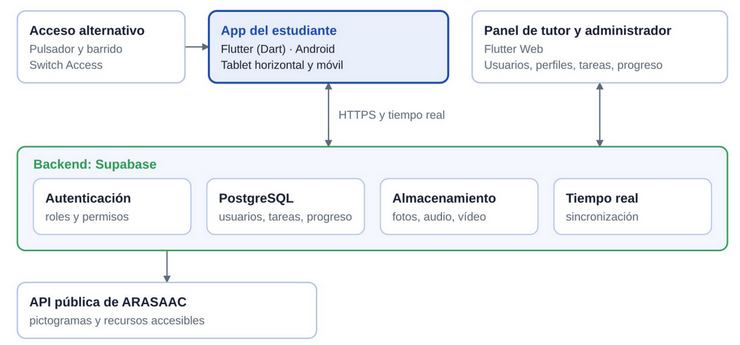
\includegraphics[width=\linewidth,height=0.42\textheight,keepaspectratio]{arquitectura.png}
\caption{Esquema general de la arquitectura del sistema propuesto}
\end{figure}

\subsection*{8.1. Tecnologías}
La tabla distingue lo que indica el pliego y lo que ha decidido el equipo. Las decisiones sobre el front-end, el hosting y el backend constan en el acta del 8 de octubre de 2026.

\par\noindent\begin{tabular}{@{}>{\raggedright\arraybackslash}p{\dimexpr 0.2000\linewidth-2\tabcolsep\relax}>{\raggedright\arraybackslash}p{\dimexpr 0.2375\linewidth-2\tabcolsep\relax}>{\raggedright\arraybackslash}p{\dimexpr 0.2875\linewidth-2\tabcolsep\relax}>{\raggedright\arraybackslash}p{\dimexpr 0.2750\linewidth-2\tabcolsep\relax}@{}}
\rowcolor{gblue}\textcolor{white}{\textbf{Capa}} & \textcolor{white}{\textbf{Tecnología}} & \textcolor{white}{\textbf{Finalidad}} & \textcolor{white}{\textbf{Carácter}} \\
\hl{Front-end de la aplicación web} & Native & Desarrollo de una única aplicación web con la interfaz del estudiante y el panel de tutores y administrador. & Decisión del equipo (acta del 08/10/2026, A-01 y A-02) \\ \arrayrulecolor{gline}\hline
\rowcolor{glight}
\hl{Hosting} & Vercel (plan gratuito) & Publicar la aplicación web para usarla desde el navegador. & Decisión del equipo (acta del 08/10/2026, A-01) \\ \arrayrulecolor{gline}\hline
\hl{Backend} & Supabase: PostgreSQL, autenticación, almacenamiento y tiempo real & Gestión de datos, usuarios, archivos y sincronización. & Decisión del equipo (acta del 08/10/2026, A-01), a validar con un prototipo en la fase inicial \\ \arrayrulecolor{gline}\hline
\rowcolor{glight}
\hl{Pictogramas} & API pública de ARASAAC & Incorporación de pictogramas y recursos accesibles. & Indicado en el pliego \\ \arrayrulecolor{gline}\hline
\hl{Accesibilidad} & Propiedades de accesibilidad de Native; pruebas en el navegador con lector de pantalla y teclado & Implementar la accesibilidad y validarla antes de cada entrega. & Requisito a implementar y validar \\ \arrayrulecolor{gline}\hline
\rowcolor{glight}
\hl{Calidad} & ESLint, Prettier, GitHub Actions y revisión de ramas en GitHub & Mantener la calidad y consistencia del código. & Decisión del equipo (Manual de coordinación y Práctica 2) \\ \arrayrulecolor{gline}\hline
\hl{Organización de los sprints} & Jira & Product Backlog, planificación y seguimiento de cada sprint. & Decisión del equipo \\ \arrayrulecolor{gline}\hline
\rowcolor{glight}
\hl{Desarrollo y \mbox{documentación}} & VSCode, GitHub, Google Drive y LaTeX & Desarrollo, control de versiones y documentación del proyecto. & Decisión del equipo (Manual de coordinación) \\ \arrayrulecolor{gline}\hline
\end{tabular}\par\medskip
Si el prototipo de la fase inicial muestra que Supabase no se ajusta al proyecto, el equipo lo sustituirá por otra opción de software libre o con licencia universitaria. Ese cambio solo afectaría a la capa de backend.



\clearpage
\section{Actividades a realizar}
El proyecto sigue Scrum y los sprints se organizan en \hl{Jira}. Tras una fase inicial de preparación, cada iteración termina con un \hl{incremento funcional} que el profesorado y el cliente pueden probar. El reparto de actividades sigue el plan de entregas de la Práctica 2, cargado en Jira. Al inicio de cada iteración el equipo revisa y prioriza el \hl{Product Backlog}, por lo que ese reparto puede cambiar.

{\setlength{\LTleft}{0pt}\setlength{\LTright}{0pt}
\begin{longtable}{@{}>{\raggedright\arraybackslash}p{\dimexpr 0.6250\linewidth-2\tabcolsep\relax}>{\raggedright\arraybackslash}p{\dimexpr 0.2500\linewidth-2\tabcolsep\relax}>{\raggedright\arraybackslash}p{\dimexpr 0.1250\linewidth-2\tabcolsep\relax}@{}}
\rowcolor{gblue}\textcolor{white}{\textbf{Actividad}} & \textcolor{white}{\textbf{Objetivos}} & \textcolor{white}{\textbf{Etapa}} \\
\endfirsthead
\rowcolor{gblue}\textcolor{white}{\textbf{Actividad}} & \textcolor{white}{\textbf{Objetivos}} & \textcolor{white}{\textbf{Etapa}} \\
\endhead
\hl{A1. Propuesta técnica, manual de coordinación, presupuesto y planificación} & OE17 & Fase inicial \\ \arrayrulecolor{gline}\hline
\rowcolor{glight}
\hl{A2. Entrevista con el cliente, personajes, escenarios y Product Backlog inicial en Jira} & OE1-OE17 & Fase inicial \\ \arrayrulecolor{gline}\hline
\hl{A3. Formación en Native, accesibilidad y calidad; entorno de trabajo y prototipo del backend} & OE14, OE16, OE17 & Fase inicial \\ \arrayrulecolor{gline}\hline
\rowcolor{glight}
\hl{A4. Infraestructura: backend, integración continua, despliegue y componentes base accesibles} & OE14, OE16 & 1 \\ \arrayrulecolor{gline}\hline
\hl{A5. Acceso adaptado, usuarios, roles y vínculos entre tutores y estudiantes} & OE1, OE2, OE15 & 1 y 2 \\ \arrayrulecolor{gline}\hline
\rowcolor{glight}
\hl{A6. Personalización del perfil y de la interfaz; modo de barrido y vista semanal} & OE3 & 1 y 3 \\ \arrayrulecolor{gline}\hline
\hl{A7. Agenda diaria, confirmación de inicio y fin, reloj visual y avisos anticipatorios} & OE4, OE6 & 1 \\ \arrayrulecolor{gline}\hline
\rowcolor{glight}
\hl{A8. Botón de necesidades básicas; urgencias, valoración y comunicación} & OE11 & 1 y 3 \\ \arrayrulecolor{gline}\hline
\hl{A9. Tareas personales y tareas por pasos con contenido multimedia} & OE5, OE6 & 2 \\ \arrayrulecolor{gline}\hline
\rowcolor{glight}
\hl{A10. Tareas del centro: comedor, menú mensual, reprografía y guía de visita} & OE7-OE10 & 2 \\ \arrayrulecolor{gline}\hline
\hl{A11. Imprevistos: plan B, prioridad y bloqueo de tareas} & OE12 & 3 \\ \arrayrulecolor{gline}\hline
\rowcolor{glight}
\hl{A12. Seguimiento del progreso por el tutor} & OE13 & 2 y 3 \\ \arrayrulecolor{gline}\hline
\hl{A13. Auditoría de accesibilidad y pruebas con los dispositivos del centro} & OE14 & 1, 2 y 3 \\ \arrayrulecolor{gline}\hline
\rowcolor{glight}
\hl{A14. Revisión del cumplimiento del RGPD y la LOPDGDD} & OE15 & 3 \\ \arrayrulecolor{gline}\hline
\hl{A15. Planificación, revisión y retrospectiva de cada sprint en Jira, y refinamiento del Product Backlog} & OE17 & 1, 2 y 3 \\ \arrayrulecolor{gline}\hline
\rowcolor{glight}
\hl{A16. Pruebas finales, informe de calidad y presentación final} & OE17 & 3 \\ \arrayrulecolor{gline}\hline
\end{longtable}}
\needspace{14\baselineskip}
\section{Cronograma}
En cada iteración coordinan dos integrantes, rotando entre Juan Luis, Germán, Jaime y Ana. El gestor de calidad (Javier) y el gestor de usabilidad y accesibilidad (Álvaro) revisan todas las entregas. Cada iteración corresponde a un sprint de Jira; entre paréntesis se indican los puntos de historia (SP) planificados en la Práctica 2. El diagrama de Gantt, los entregables y los hitos están en el documento Propuesta de solución.

\par\noindent\begin{tabular}{@{}>{\raggedright\arraybackslash}p{\dimexpr 0.1313\linewidth-2\tabcolsep\relax}>{\raggedright\arraybackslash}p{\dimexpr 0.1500\linewidth-2\tabcolsep\relax}>{\raggedright\arraybackslash}p{\dimexpr 0.1688\linewidth-2\tabcolsep\relax}>{\raggedright\arraybackslash}p{\dimexpr 0.2375\linewidth-2\tabcolsep\relax}>{\raggedright\arraybackslash}p{\dimexpr 0.3125\linewidth-2\tabcolsep\relax}@{}}
\rowcolor{gblue}\textcolor{white}{\textbf{Etapa}} & \textcolor{white}{\textbf{Fechas}} & \textcolor{white}{\textbf{Actividades}} & \textcolor{white}{\textbf{Incremento funcional}} & \textcolor{white}{\textbf{Entregables}} \\
\hl{Fase inicial} & 1-21 oct. 2026 & A1-A3 & Prototipo del entorno y del backend & Propuesta técnica, manual de coordinación, presupuesto, planificación, personajes y escenarios, Product Backlog inicial \\ \arrayrulecolor{gline}\hline
\rowcolor{glight}
\hl{Iteración 1} (34 SP) & 22-23 oct. a 11-12 nov. 2026 & A4-A8, A13, A15 & Acceso adaptado, perfiles y personalización, agenda «Hecho, Ahora, Después», reloj visual, avisos anticipatorios y botón de necesidades & Incremento 1, especificación de requisitos, historias con tareas y pruebas de aceptación, informes de evaluación y retrospectiva, presentación \\ \arrayrulecolor{gline}\hline
\hl{Iteración 2} (29 SP) & 12-13 nov. a 2-3 dic. 2026 & A5, A9, A10, A12, A13, A15 & Tareas personales y por pasos, y tareas del centro: comedor, menú mensual, reprografía y guía de visita & Incremento 2, análisis y diseño, arquitectura, informes de evaluación y retrospectiva, presentación de iteración y al cliente \\ \arrayrulecolor{gline}\hline
\rowcolor{glight}
\hl{Iteración 3} (23 SP) & 3-4 dic. a 16 dic. 2026 & A6, A8, A11-A16 & Plan B y bloqueo de tareas, urgencias y comunicación, modo de barrido, vista semanal y seguimiento semanal & Aplicación final, pruebas, informe de usabilidad y accesibilidad, informe de calidad, código documentado, presentación final \\ \arrayrulecolor{gline}\hline
\end{tabular}\par\medskip
La entrega oficial de la tercera iteración es el 21 de diciembre de 2026; el equipo cierra el 16 para disponer de margen.

\needspace{10\baselineskip}
\section{Cauces de seguimiento}
El cliente podrá conocer el estado y evolución del proyecto mediante diferentes mecanismos de seguimiento, respetando las directrices establecidas por el profesorado para la comunicación con el Colegio:

\begin{itemize}
\item \hl{Reuniones semanales con el profesorado}, durante las clases de prácticas, para informar sobre el estado del proyecto, las tareas realizadas, el tiempo dedicado y las posibles dificultades.
\item \hl{Reuniones periódicas con el Colegio}, comenzando por la entrevista inicial de requisitos, para revisar el trabajo y validar los prototipos.
\item \hl{Revisión de cada incremento funcional} al final de cada iteración y \hl{presentaciones al finalizar la primera y la segunda iteración}, mostrando las funcionalidades desarrolladas.
\item \hl{Presentación al cliente a mitad del proyecto}, en la fecha que se determine.
\item \hl{Informes de estado por iteración}, incluyendo el progreso respecto a la planificación, riesgos identificados y cambios realizados.
\item \hl{Tablero de Jira accesible al profesorado}, donde podrán consultarse el Product Backlog, el sprint en curso y el gráfico de evolución.
\item \hl{Repositorio de GitHub accesible al profesorado}, donde podrá consultarse la evolución del código y la documentación.
\item \hl{Aplicación web publicada en Vercel}, que permite probar cada incremento desde el navegador.
\item \hl{Comunicación de posibles retrasos con al menos tres días de antelación}, justificando las causas y actualizando la planificación correspondiente.
\end{itemize}
\needspace{12\baselineskip}
\section{Valor añadido}
Son características que el cliente no ha pedido y que el equipo incorpora a partir del estudio etnográfico (apartado 6):

\begin{itemize}
\item \hl{Refuerzo positivo} al completar una tarea, configurable por perfil (RF6.5).
\item \hl{Avisos solo visuales y reloj silencioso} para el alumnado con molestia ante los sonidos (RF3.9, RF3.11).
\item \hl{Rótulo en Lectura Fácil} bajo el reloj visual con el tiempo que queda (RF6.7).
\item \hl{Asistente para crear tareas sin escribir}, con pictogramas, audio, vídeo y selección visual de días y horas (RF5.10).
\item \hl{Lectura en voz alta} de las tareas y los pasos (RF14.5).
\item \hl{Indicador de foco configurable} por perfil, visible solo cuando el estudiante lo necesita (RF14.4).
\item \hl{Biblioteca de recursos accesibles} que comprueba que cada recurso tiene su descripción (RF14.6, RF14.7).
\item \hl{Separación entre tareas del centro y del hogar}, con permisos distintos para tutores escolares y familiares (RF2.12, RF2.13, RF15.2).
\item \hl{Códigos QR imprimibles} para las salas de la guía de visita (RF10.5, RF10.6).
\item \hl{Exportación del parte de comedor} por el personal de cocina (RF8.10).
\item \hl{Sin instalación:} al ser una aplicación web, funciona en cualquier dispositivo con navegador y se actualiza para todos a la vez (RF16.1).
\end{itemize}
\needspace{14\baselineskip}
\section{Beneficios y beneficiarios}
Los beneficiarios \hl{directos} usan la aplicación; los \hl{indirectos} se benefician de su uso sin manejarla a diario. Las cifras que no constan en la documentación están pendientes de confirmar con el Colegio.

{\small\par\noindent\begin{tabular}{@{}>{\raggedright\arraybackslash}p{\dimexpr 0.2500\linewidth-2\tabcolsep\relax}>{\raggedright\arraybackslash}p{\dimexpr 0.1200\linewidth-2\tabcolsep\relax}>{\raggedright\arraybackslash}p{\dimexpr 0.1800\linewidth-2\tabcolsep\relax}>{\raggedright\arraybackslash}p{\dimexpr 0.4500\linewidth-2\tabcolsep\relax}@{}}
\rowcolor{gblue}\textcolor{white}{\textbf{Beneficiario}} & \textcolor{white}{\textbf{Tipo}} & \textcolor{white}{\textbf{Cuántos}} & \textcolor{white}{\textbf{Beneficio principal}} \\
\hl{Estudiantes del PTVAL} & Directo & Pendiente de confirmar & Más autonomía en las tareas del centro y del hogar y menos ansiedad ante el tiempo y los imprevistos. \\ \arrayrulecolor{gline}\hline
\rowcolor{glight}
\hl{Tutores de aula} & Directo & Pendiente de confirmar & Menos acompañamiento físico e instrucciones repetidas; perfiles configurables y seguimiento del progreso. \\ \arrayrulecolor{gline}\hline
\hl{Familias y tutores legales} & Directo & Uno por estudiante & Programar tareas del hogar y consultar su realización con la misma herramienta. \\ \arrayrulecolor{gline}\hline
\rowcolor{glight}
\hl{Administración del Colegio} & Directo & Pendiente de confirmar & Gestión centralizada de usuarios, tareas y recursos, con control de los datos personales. \\ \arrayrulecolor{gline}\hline
\hl{Personal de cocina y reprografía} & Indirecto & Pendiente de confirmar & Partes y encargos ordenados y menos errores de transcripción. \\ \arrayrulecolor{gline}\hline
\rowcolor{glight}
\hl{Especialistas y terapeutas} & Indirecto & Pendiente de confirmar & Información del progreso y de las valoraciones del estudiante. \\ \arrayrulecolor{gline}\hline
\hl{Equipo y profesorado de DGP y MDA} & Indirecto & 6 estudiantes y el profesorado de ambas asignaturas & Experiencia en un proyecto real de aprendizaje-servicio dentro de AUTOVIDA. \\ \arrayrulecolor{gline}\hline
\end{tabular}\par}\medskip

\needspace{12\baselineskip}
\subsection*{13.1. Propiedad de la aplicación y explotación}
El equipo \hl{Los Gantt-sters conserva la propiedad intelectual de TuAgendita}: el código fuente, el diseño, la marca y la documentación. Lo que se cede a cada centro es una \hl{licencia de uso no exclusiva}, no la propiedad de la aplicación.

\begin{itemize}
\item \hl{Modalidades de licencia:} pago único (precio fijo) o cuota periódica (mensualidad), a elección de cada centro.
\item \hl{Sin exclusividad:} aunque un centro adquiera la aplicación, el equipo puede seguir ofreciéndola y vendiéndola a otros colegios, asociaciones y entidades.
\item \hl{Datos de cada centro:} los datos personales del alumnado pertenecen a cada centro, que es su responsable de tratamiento; la licencia no da al equipo derecho a usarlos para otros fines (RGPD).
\end{itemize}
\hl{A tener en cuenta:} el pliego (apartado 5) establece que los productos de esta licitación son propiedad de los equipos y de los peticionarios, con autoría compartida, por lo que la venta a terceros deberá acordarse con el profesorado y el Colegio. Además, los pictogramas de ARASAAC tienen licencia CC BY-NC-SA, que no permite el uso comercial; una versión de pago tendrá que pedir autorización a ARASAAC o sustituir esos pictogramas.

\bloque{Beneficio para el equipo}
Conservar la propiedad permite adaptar la aplicación a otros centros de educación especial con programas de transición a la vida adulta y obtener ingresos de cada licencia. Es una previsión de negocio, no un requisito de este proyecto.

\end{document}
